
%%% Local Variables:
%%% mode: latex
%%% TeX-master: t
%%% End:
\documentclass{beamerthemeMono}

% specify some optional logos
\graphicspath{{figures/}}
\pgfdeclareimage[height=1.45cm]{mainlogo}{figures/logo}
\logo{\pgfuseimage{mainlogo}}
% placed in the lower left/right corner if the \pgfuseimage{minilogo}
% command is uncommented in the \institute command below.
\pgfdeclareimage[height=0.3cm]{minilogo}{figures/logo}

\AtBeginSection[] {
  \begin{frame}
    \frametitle{目录}
    {\tableofcontents[%
      currentsection, % causes all sections but the current to be shown in a semi-transparent way.
%     currentsubsection, % causes all subsections but the current subsection in the current section to ...
      hideallsubsections % causes all subsections to be hidden.
%     hideothersubsections, % causes the subsections of sections other than the current one to be hidden.
%     part=, % part number causes the table of contents of part part number to be shown
%     pausesections, % causes a \pause command to be issued before each section. This is useful if you
%     pausesubsections, %  causes a \pause command to be issued before each subsection.
%     sections={ overlay specification },
      ]}
   \end{frame}}
%%%%%%%%%%%%%%%%%%%%%%%%%%%%%%%%%%%%%%%%%%%%%%%%%%%%%%%%%%%%
%%%%%%%%%%%%%%%%%%%%%%%%%%%%%%%%%%%%%%%%%%%%%%%%%%%%%%%%%%%%
          % 文档开始
%%%%%%%%%%%%%%%%%%%%%%%%%%%%%%%%%%%%%%%%%%%%%%%%%%%%%%%%%%%%
%%%%%%%%%%%%%%%%%%%%%%%%%%%%%%%%%%%%%%%%%%%%%%%%%%%%%%%%%%%%

 \begin{document}

 \title[统计图形和R]% optional, use only with long paper titles
 {\erhao 统计图形和R\\[2ex]}

 \author[邹海翔] % optional, use only with lots of authors
 {邹海翔}

 % - Give the names in the same order as they appear in the paper.  -
 % Use the \inst{?} command only if the authors have different
 % affiliation. See the beamer manual for an example


 \institute[深圳市规划国土发展研究中心] % optional - is placed in the bottom of the sidebar on every slide
 {%
   \wuhao 深圳市规划国土发展研究中心
   % there must be an empty line above this line - otherwise some
   % unwanted space is added
   % between the university and the country (I do not know why;( )
 }

 % \date{\today}
 \date{2017 年 12 月}
 \titlegraphic{\pgfuseimage{mainlogo}} %insert a company or department logo


 % the titlepage the plain option removes the sidebar and header from
 % the title page
 \begin{frame}[plain]
   \titlepage
 \end{frame}
%%%%%%%%%%%%%%%%

 % TOC
 \begin{frame}{大纲}{}
   {\tableofcontents[hideallsubsections]}
 \end{frame}

%%%%%%%%%%%%%%%%%%%%%%%%%%%%%%%%%%%%%%%%%%%%%%%%%%%%%%%%%%%%
 \section{统计图形}
%%%%%%%%%%%%%%%%
 \subsection{线图}

 \begin{frame}[c]{线图(line chart)}{}

\begin{overlayarea}  {\textwidth}{\textheight}
  \only<1>{
    \begin{figure}
      \centering
      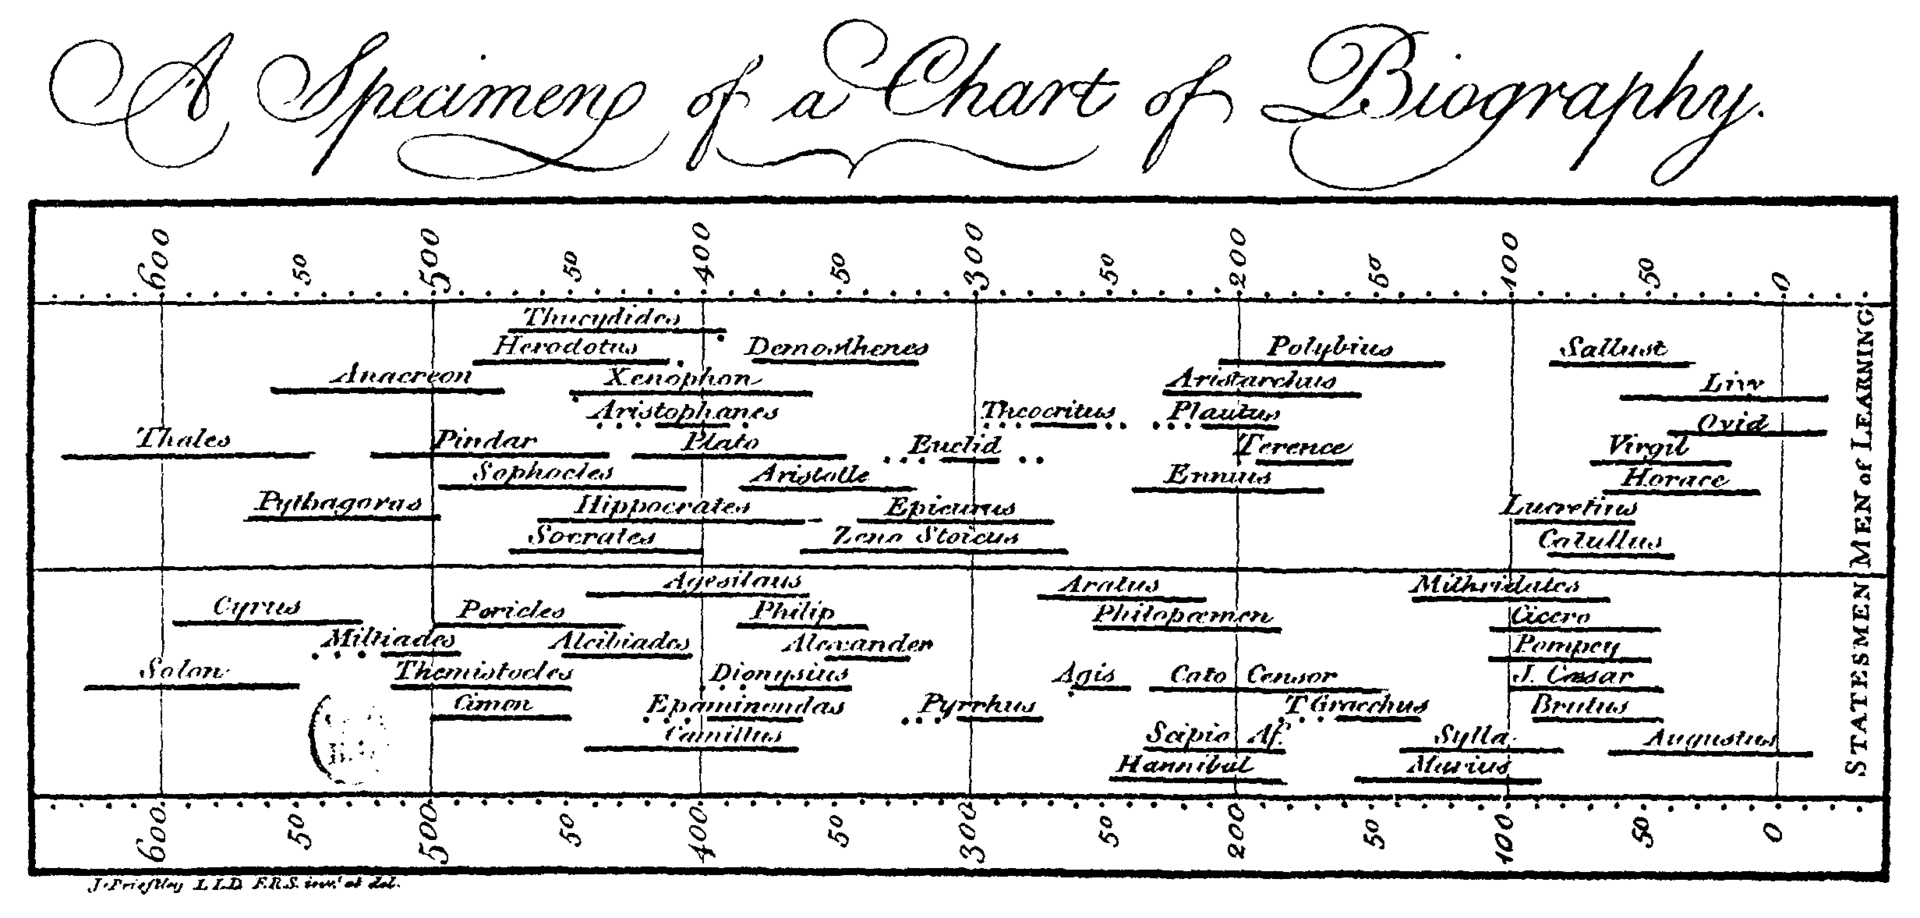
\includegraphics[width=\textwidth]{Priestley_Chart.png}
      \caption{英国化学家Joseph Priestley于1765年绘制的时间线图
        是\emphText{历史上最早的统计图形},这幅图展示了多个历史人物在历
        史长河中的跨度}
    \end{figure}} \only<2>{
    \begin{figure}
      \centering
      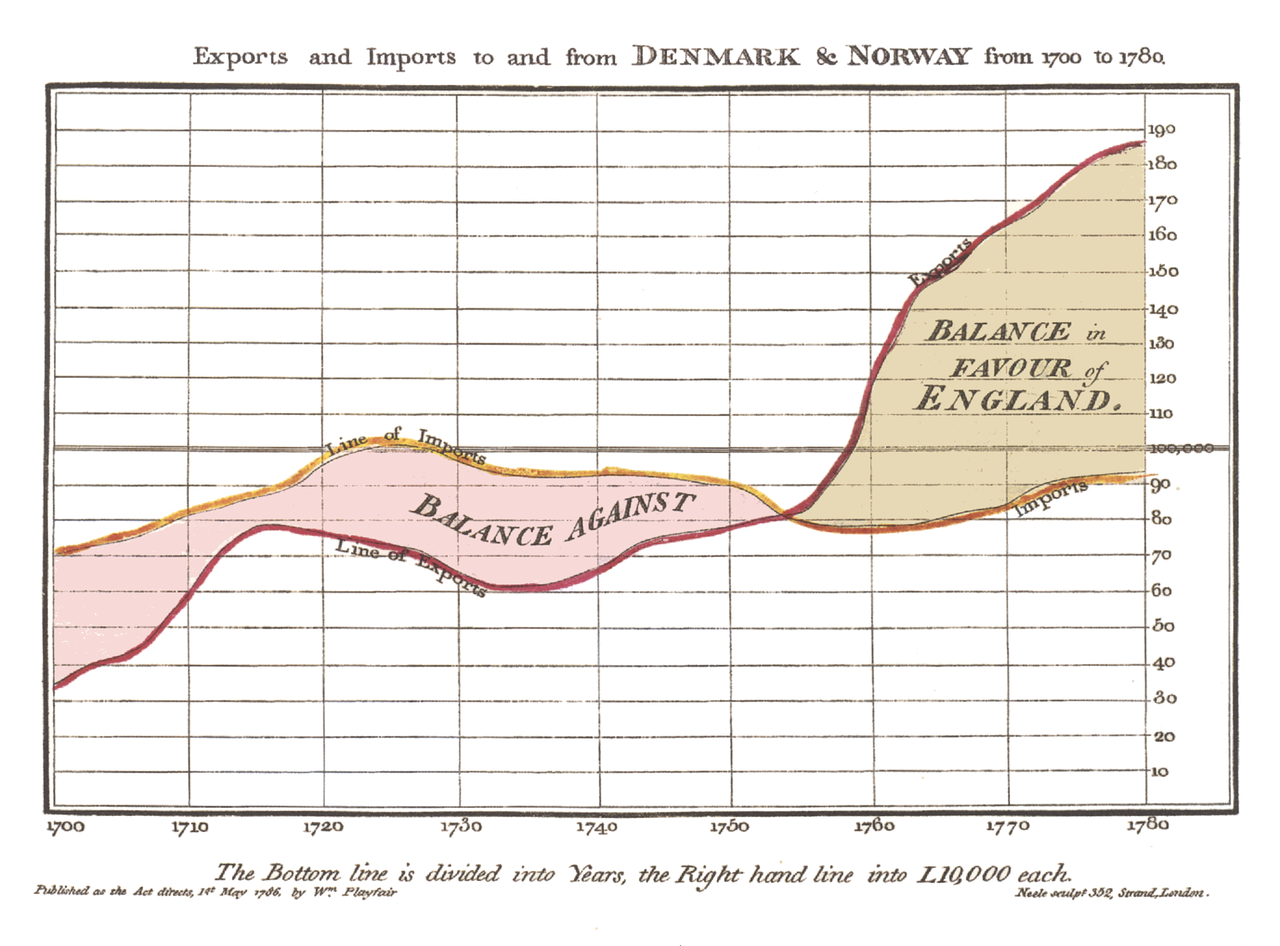
\includegraphics[width=0.75\textwidth]{Playfair_TimeSeries.png}
      \caption{苏格兰工程师和政治经济学家William Playfair于1786年在《Commercial and Political Atlas》
        一书中绘制的线图,这幅图展示了1700年至1780年间英格兰的进出口时序数据。\emphText{Playfair是历史上第一个系统使用统计图形的人,被称为“统计图形奠基人”}}
    \end{figure}}
\end{overlayarea}
 
\end{frame}

\subsection{柱状图}

\begin{frame}[c]{柱状图(bar chart)}{}

  \begin{figure}
    \centering
    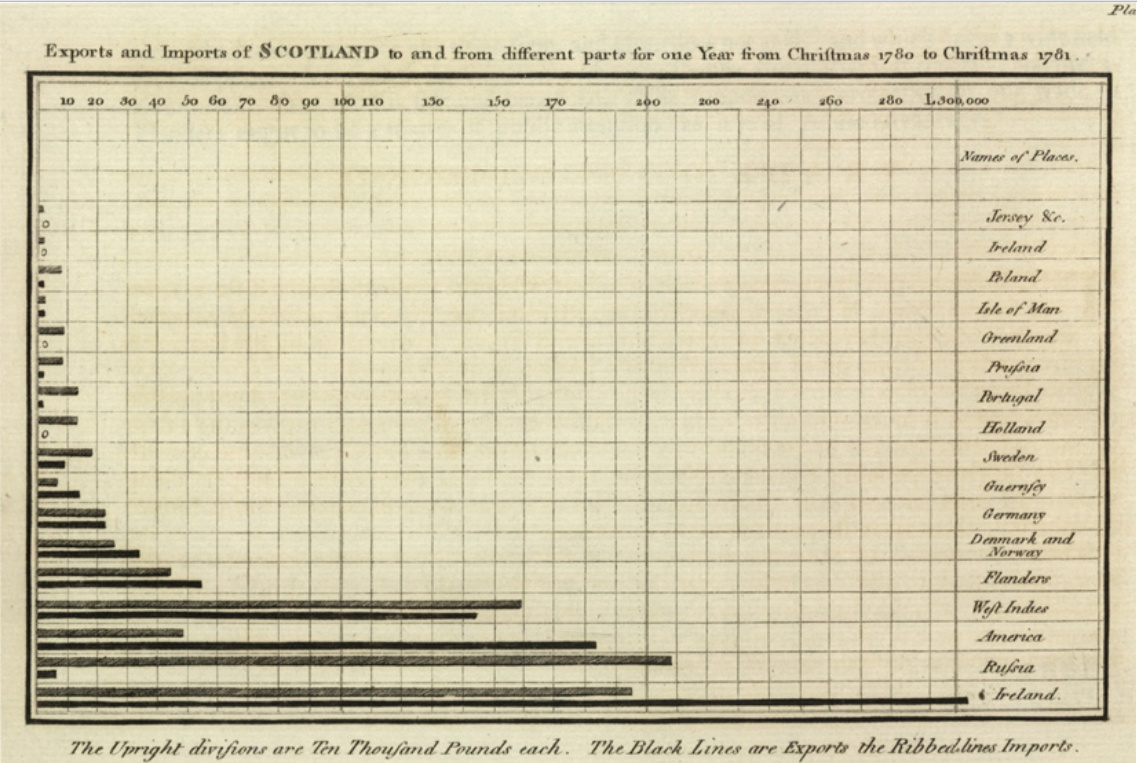
\includegraphics[width=0.8\textwidth]{Playfair_barchart.jpg}
    \caption{受到Priestley时间线图的影响,Playfair于1786年同样在
      《Commercial and Political Atlas》这本书中绘制了\emphText{历史上
        最早的柱状图},这幅图展示了不同国家的进出口数据}
  \end{figure}

\end{frame}

\subsection{饼图}

\begin{frame}[c]{饼图(pie chart)}{}

  \begin{figure}
    \begin{columns}
      \begin{column}{.6\textwidth}
        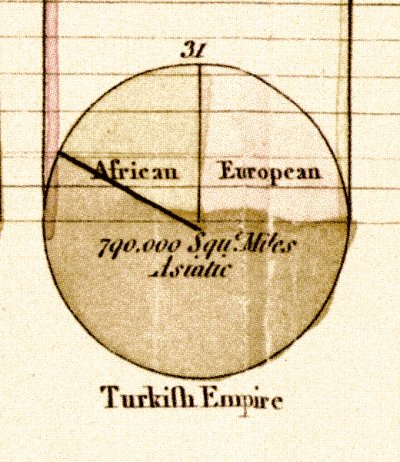
\includegraphics[width=\textwidth]{Playfair_piechart.jpg}
      \end{column}

    \begin{column}{.35\textwidth}
      \centering
      \caption{Playfair于1801年在《Statistical Breviary》这本书中绘制
        了\emphText{历史上第一幅饼图},这幅图展示了土耳其帝国在三大洲的
        国土面积分布情况}
    \end{column}
  \end{columns}
\end{figure}

\end{frame}

\subsection{主题统计地图}
\begin{frame}{\subsecname}{法国文盲率分布图}

  \begin{figure}
    \begin{columns}
      \begin{column}{.6\textwidth}
        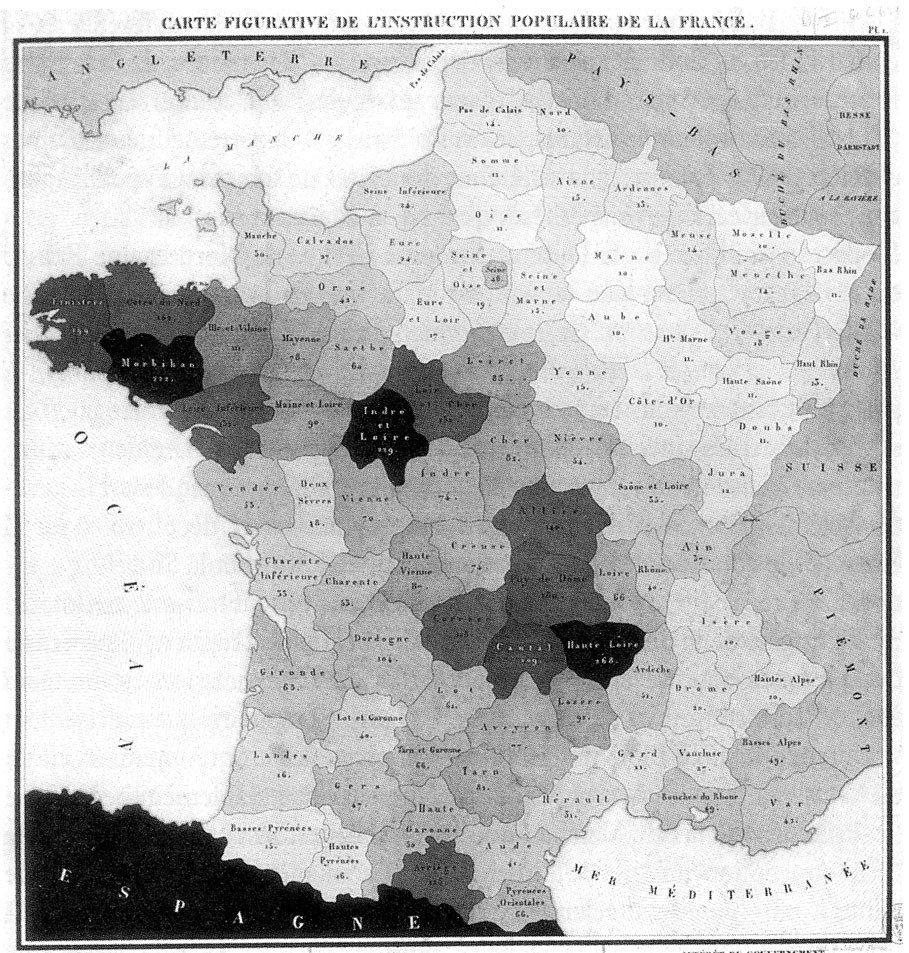
\includegraphics[width=\columnwidth]{法国文盲分布图.jpg}
      \end{column}

      \begin{column}{.35\textwidth}
        \centering
        \caption{法国文盲分布图(Charles Dupin, 1826). \\
          Charles Dupin是法国数学家,工程师,经济学家以及政客。1826年,
          他首次运用区域灰度地图的表现手段来展示法国当时的文盲率分布情
          况,\emphText{这是第一张现代形式的主题统计地图}}
      \end{column}
    \end{columns}
  \end{figure}

\end{frame}

\begin{frame}{\subsecname}{拿破仑东征图}

  \begin{figure}
    \centering 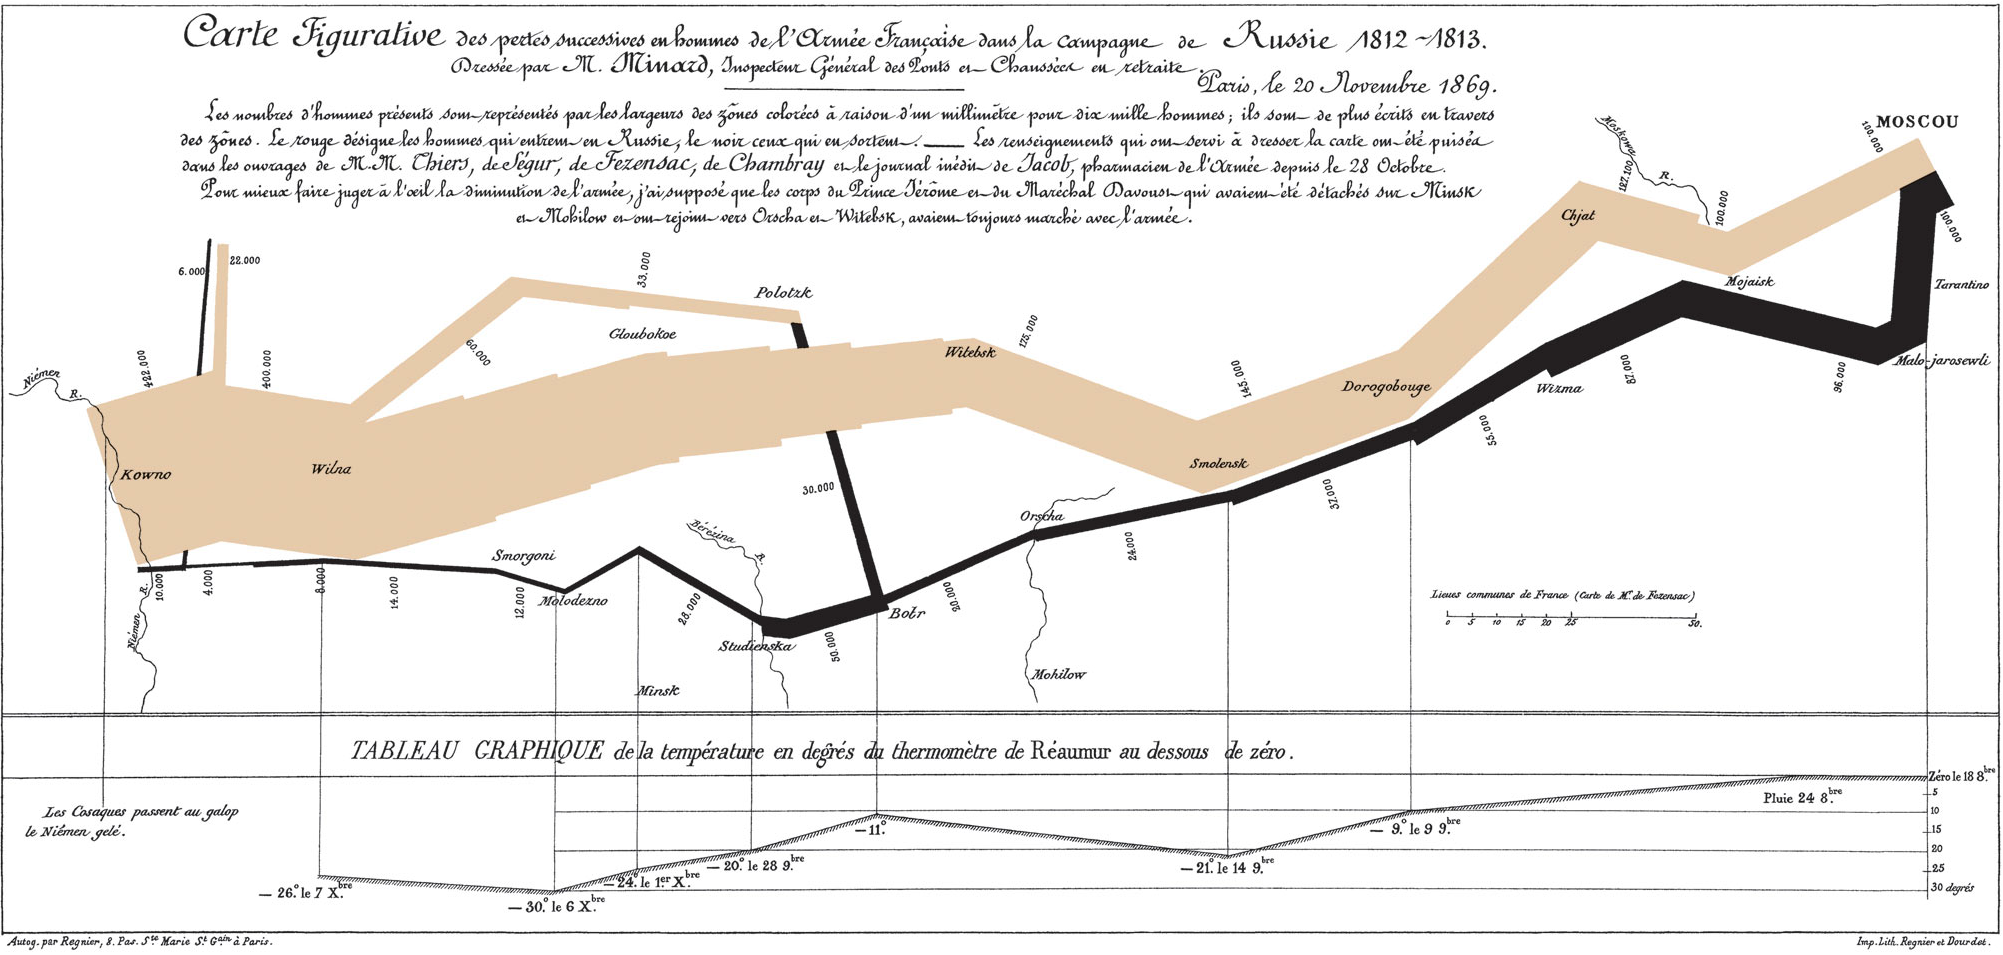
\includegraphics[width=0.8\columnwidth]{Minard.png}
    \caption{拿破仑东征图(Charles Joseph Minard, 1861). \\
      1861年,由法国工程师 Charles Joseph Minard 绘制,描述了1812年拿破
      仑东征俄罗斯的失败战役。图中同时包含了多个信息,粗细代表军队规模,
      配合日期标明了军队位置经纬度,棕色进军黑色撤退,下方折线展现气温,
      另标注了战斗的关键事件等。\\这幅图形在统计图形界内享有至高无上的
      地位,经常被一些统计、设计课程当作教学案例,被Edward
      Tufte\footnotemark[1]誉为\emphText{“有史以来最好的统计图形”}}
  \end{figure}
  \footnotetext[1]{Tufte是统计图形和信息可视化领域的领军人物,人称“数据
    达芬奇”}

\end{frame}

\begin{frame}{\subsecname}{汉尼拔远征图}

 \begin{figure}
   \centering 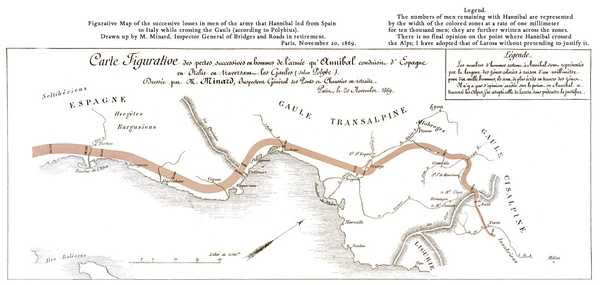
\includegraphics[width=\columnwidth]{汉尼拔远征图.jpg}
   \caption{汉尼拔远征图(Charles Joseph Minard, 1861)}
 \end{figure}

\end{frame}

\begin{frame}{\subsecname}{法国各地向巴黎输送牲畜产品的分布情况图}

  \begin{figure}
    \begin{columns}
      \begin{column}{.6\textwidth}
        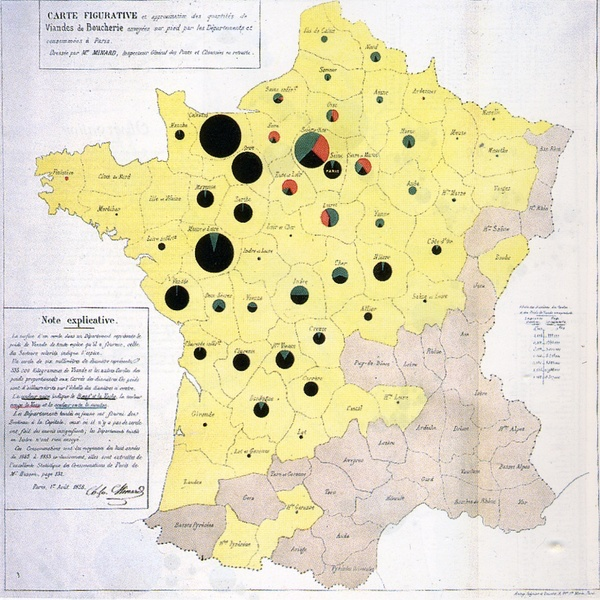
\includegraphics[width=\columnwidth]{法国各地向巴黎输送牲畜产品的分布情况图.jpg}
      \end{column}

      \begin{column}{.35\textwidth}
        \centering
        \caption{法国各地向巴黎输送牲畜产品的分布情况图(Charles Joseph Minard, 1858)\\
          此图的作者也是Joseph Minard,\emphText{经典之处在于首次将饼图融合到地图中}\\
          这位法国工程师,将一生大部分时间都贡献给了水坝,运河和桥梁的
          工程建造与教育事业,直到1851年退休,已近70岁高龄才正式开始研究数据信息图形可视化。在他最后的20年
          里,Minard在这个领域贡献了许多创新,共绘制了51幅各种形式的
          可视化图形,是那个可视化黄金时代当之无愧的大师,\emphText{被
            称为法国的“William Playfair”}}
      \end{column}
    \end{columns}
  \end{figure}

\end{frame}

\begin{frame}{\subsecname}{美国内战对欧洲棉花贸易的影响}

 \begin{figure}
   \centering 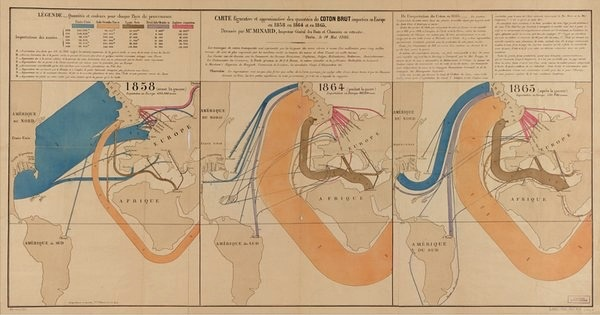
\includegraphics[width=\columnwidth]{美国内战对欧洲棉花贸易的影响.jpg}
   \caption{美国内战对欧洲棉花贸易的影响(Charles Joseph Minard, 1865)}
 \end{figure}

\end{frame}

\begin{frame}{\subsecname}{法国红酒出口情况}

 \begin{figure}
   \centering 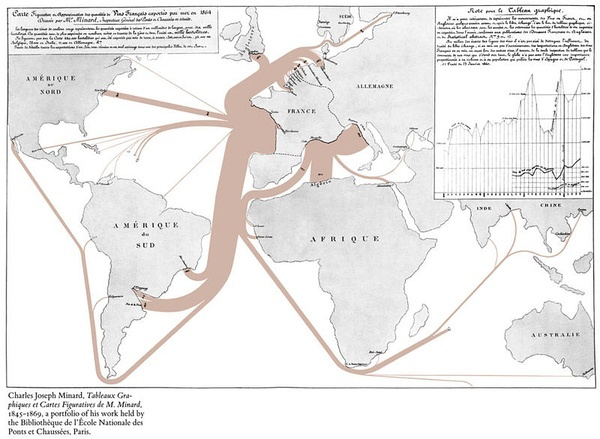
\includegraphics[width=0.8\columnwidth]{法国红酒出口情况.jpg}
   \caption{美国内战对欧洲棉花贸易的影响法国红酒出口情况(Charles
     Joseph Minard, 1864)}
 \end{figure}

\end{frame}

\begin{frame}{\subsecname}{地铁路线图}
  
  \begin{figure}\centering
    \subfloat[1908年版]
    {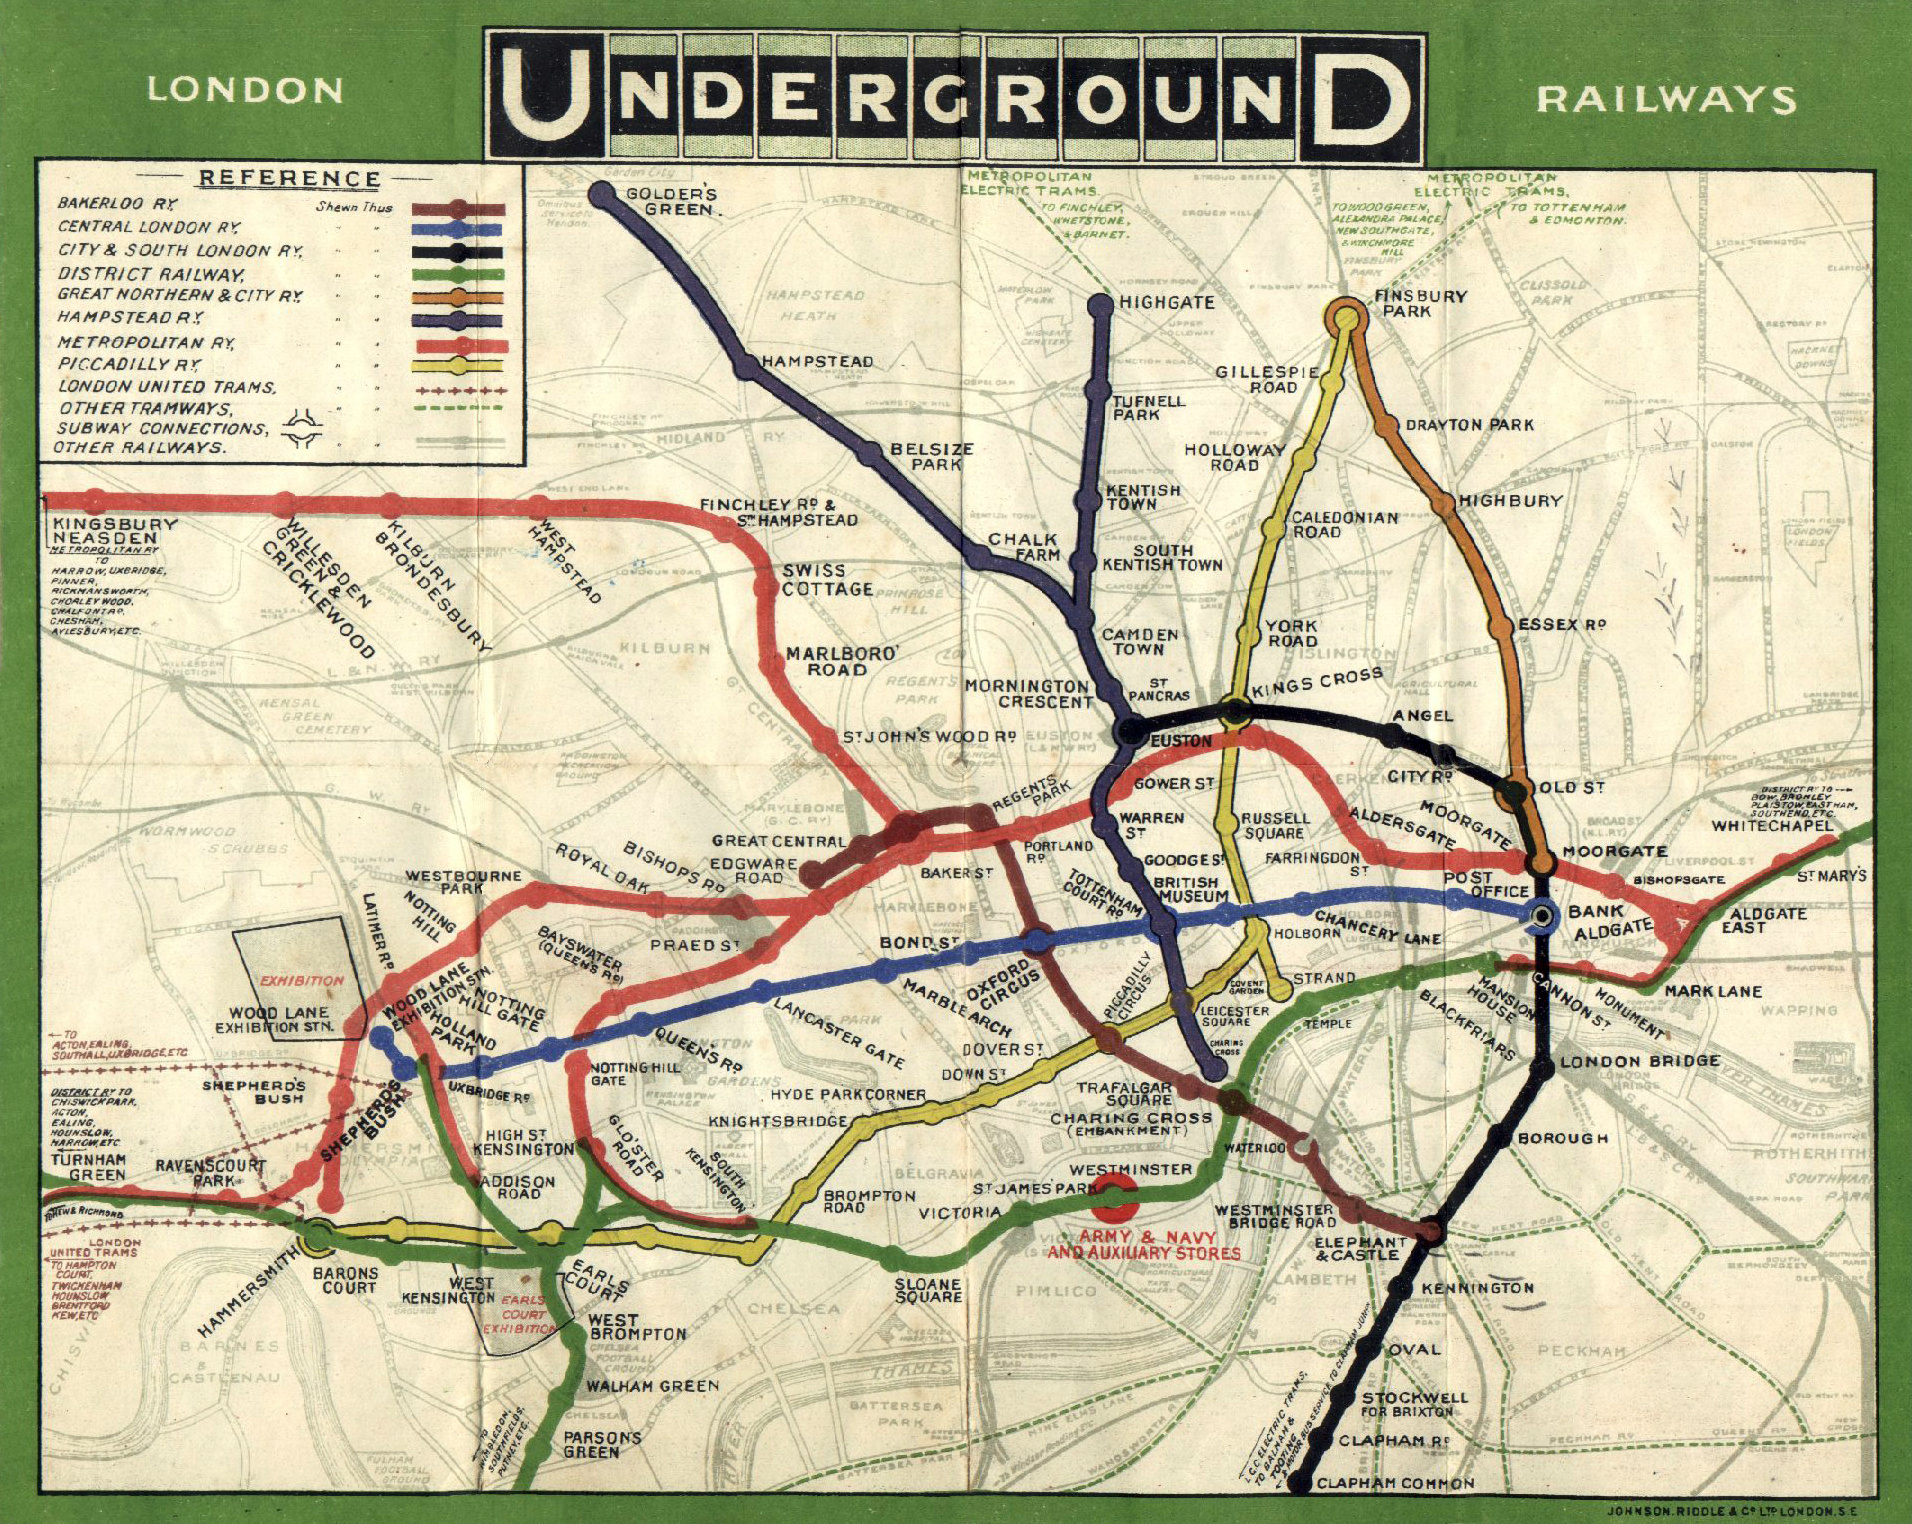
\includegraphics[width=0.45\columnwidth]{1908年伦敦地铁路线图.jpg}}\vspace{0.5pt} \subfloat[1933年版]
    {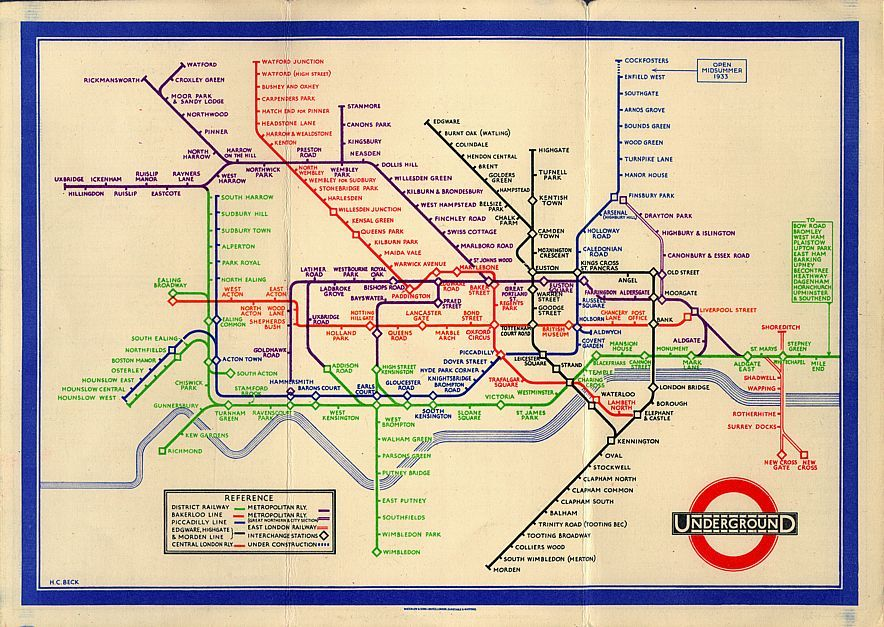
\includegraphics[width=0.45\columnwidth] {1931年贝克设计的伦敦地铁路线图.jpg}}
    \caption{道路网络形状更新在最早的地图中都是按照实地比例进行绘制的,
      比如左图的1908版伦敦地铁线路图。1931年,英国技术制图员Harry
      Beck在替伦敦地铁的讯号室绘制电路图时受到启发,设计出了经典
      的1933年版路线图(右图)}
  \end{figure}
  
\end{frame}

\begin{frame}{\subsecname}{变形地图(cartogram)}
  
  \begin{figure}\centering
    \subfloat[普通色块地图表达]
    {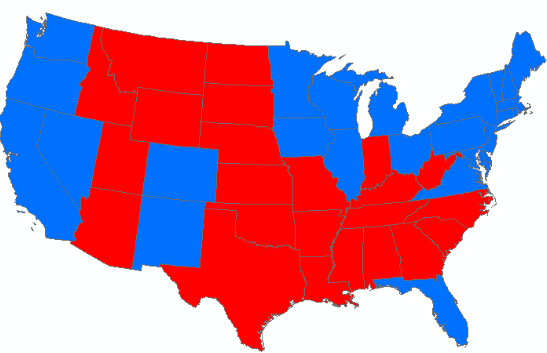
\includegraphics[width=0.45\columnwidth]{cartogram1.png}}\vspace{0.5pt}
    \subfloat[变形地图表达]
    {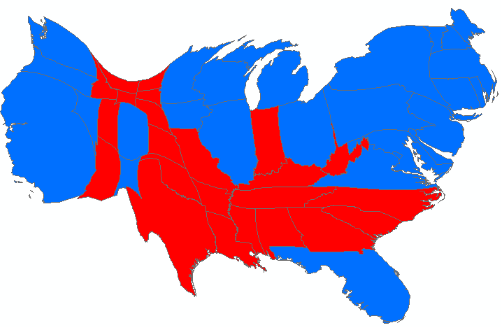
\includegraphics[width=0.45\columnwidth]{cartogram2.png}}
    \caption{变形地图的历史可以追溯到1868年,\emphText{其作用是用夸张的地图变形来表达真实的数量关系}\\上面左图是2012年
      美国大选的结果,从普通色块图上看似乎是红色代表的罗姆尼获胜,但其实获胜的是蓝色代表的奥巴马;右图是根据选票
      数量进行变形处理后的地图,可以很清楚看到蓝色多于红色,这才是真实数量的正确表达!}
  \end{figure}
  
\end{frame}

\subsection{统计图形的应用}
\begin{frame}{\subsecname}{南丁格尔玫瑰图}

 \begin{figure}
   \centering
   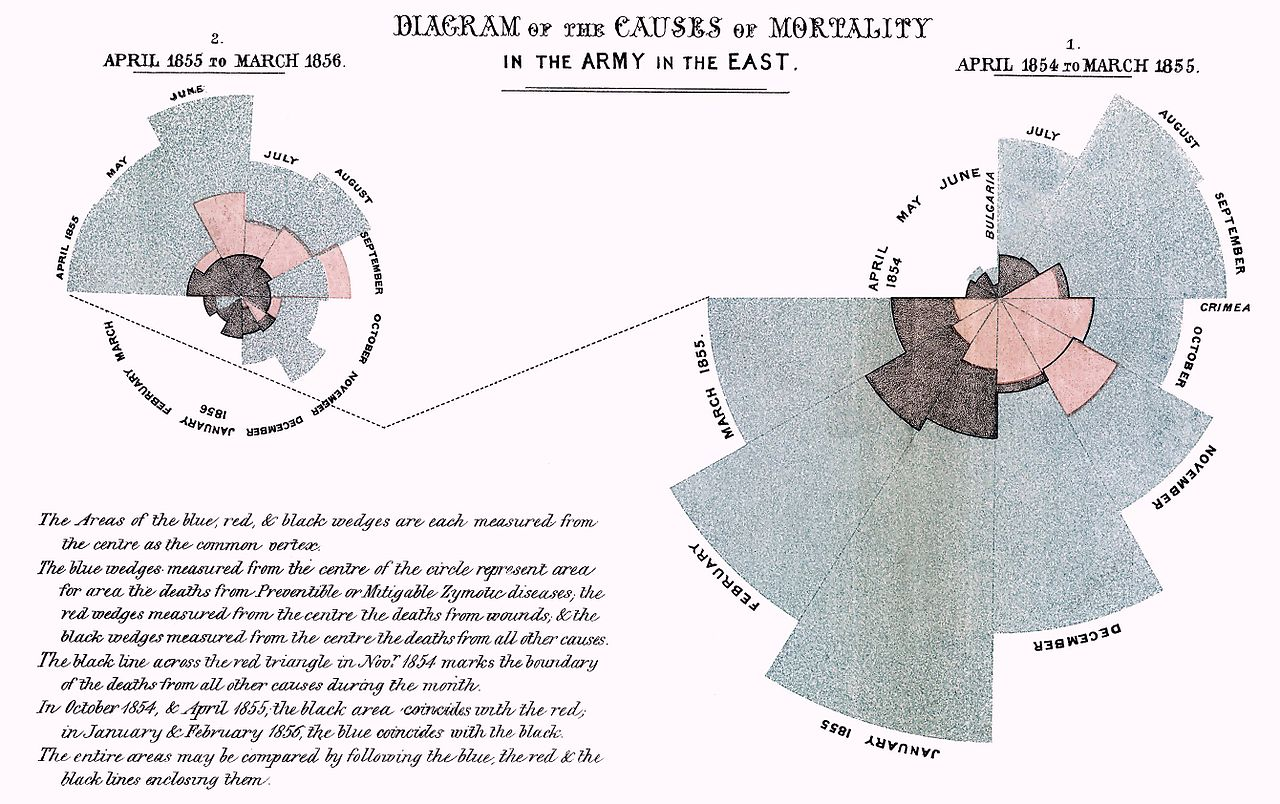
\includegraphics[width=0.8\columnwidth]{Nightingale_mortality.jpg}
   \caption{上图是南丁格尔玫瑰图。两幅图分别表示1854年和1855年军队的伤
     亡人数,
     一年12个月在极坐标上被分为12等分,每一个花瓣表示一个月;不同颜色表示死亡原因\\
     南丁格尔通过这幅图使英国政府意识到真正影响战争伤亡的并非战争本身,
     而是由于军队缺乏有效的医疗护理。由此,英国政府于1857年开设了专门的
     军医学校,培养专门的战地医护人员,\emphText{这就是统计图形在近代护
       理学最早的应用}}
 \end{figure}
\end{frame}

\begin{frame}{\subsecname}{霍乱传播之谜}

  \begin{figure}
    \begin{columns}
      \begin{column}{.6\textwidth}
        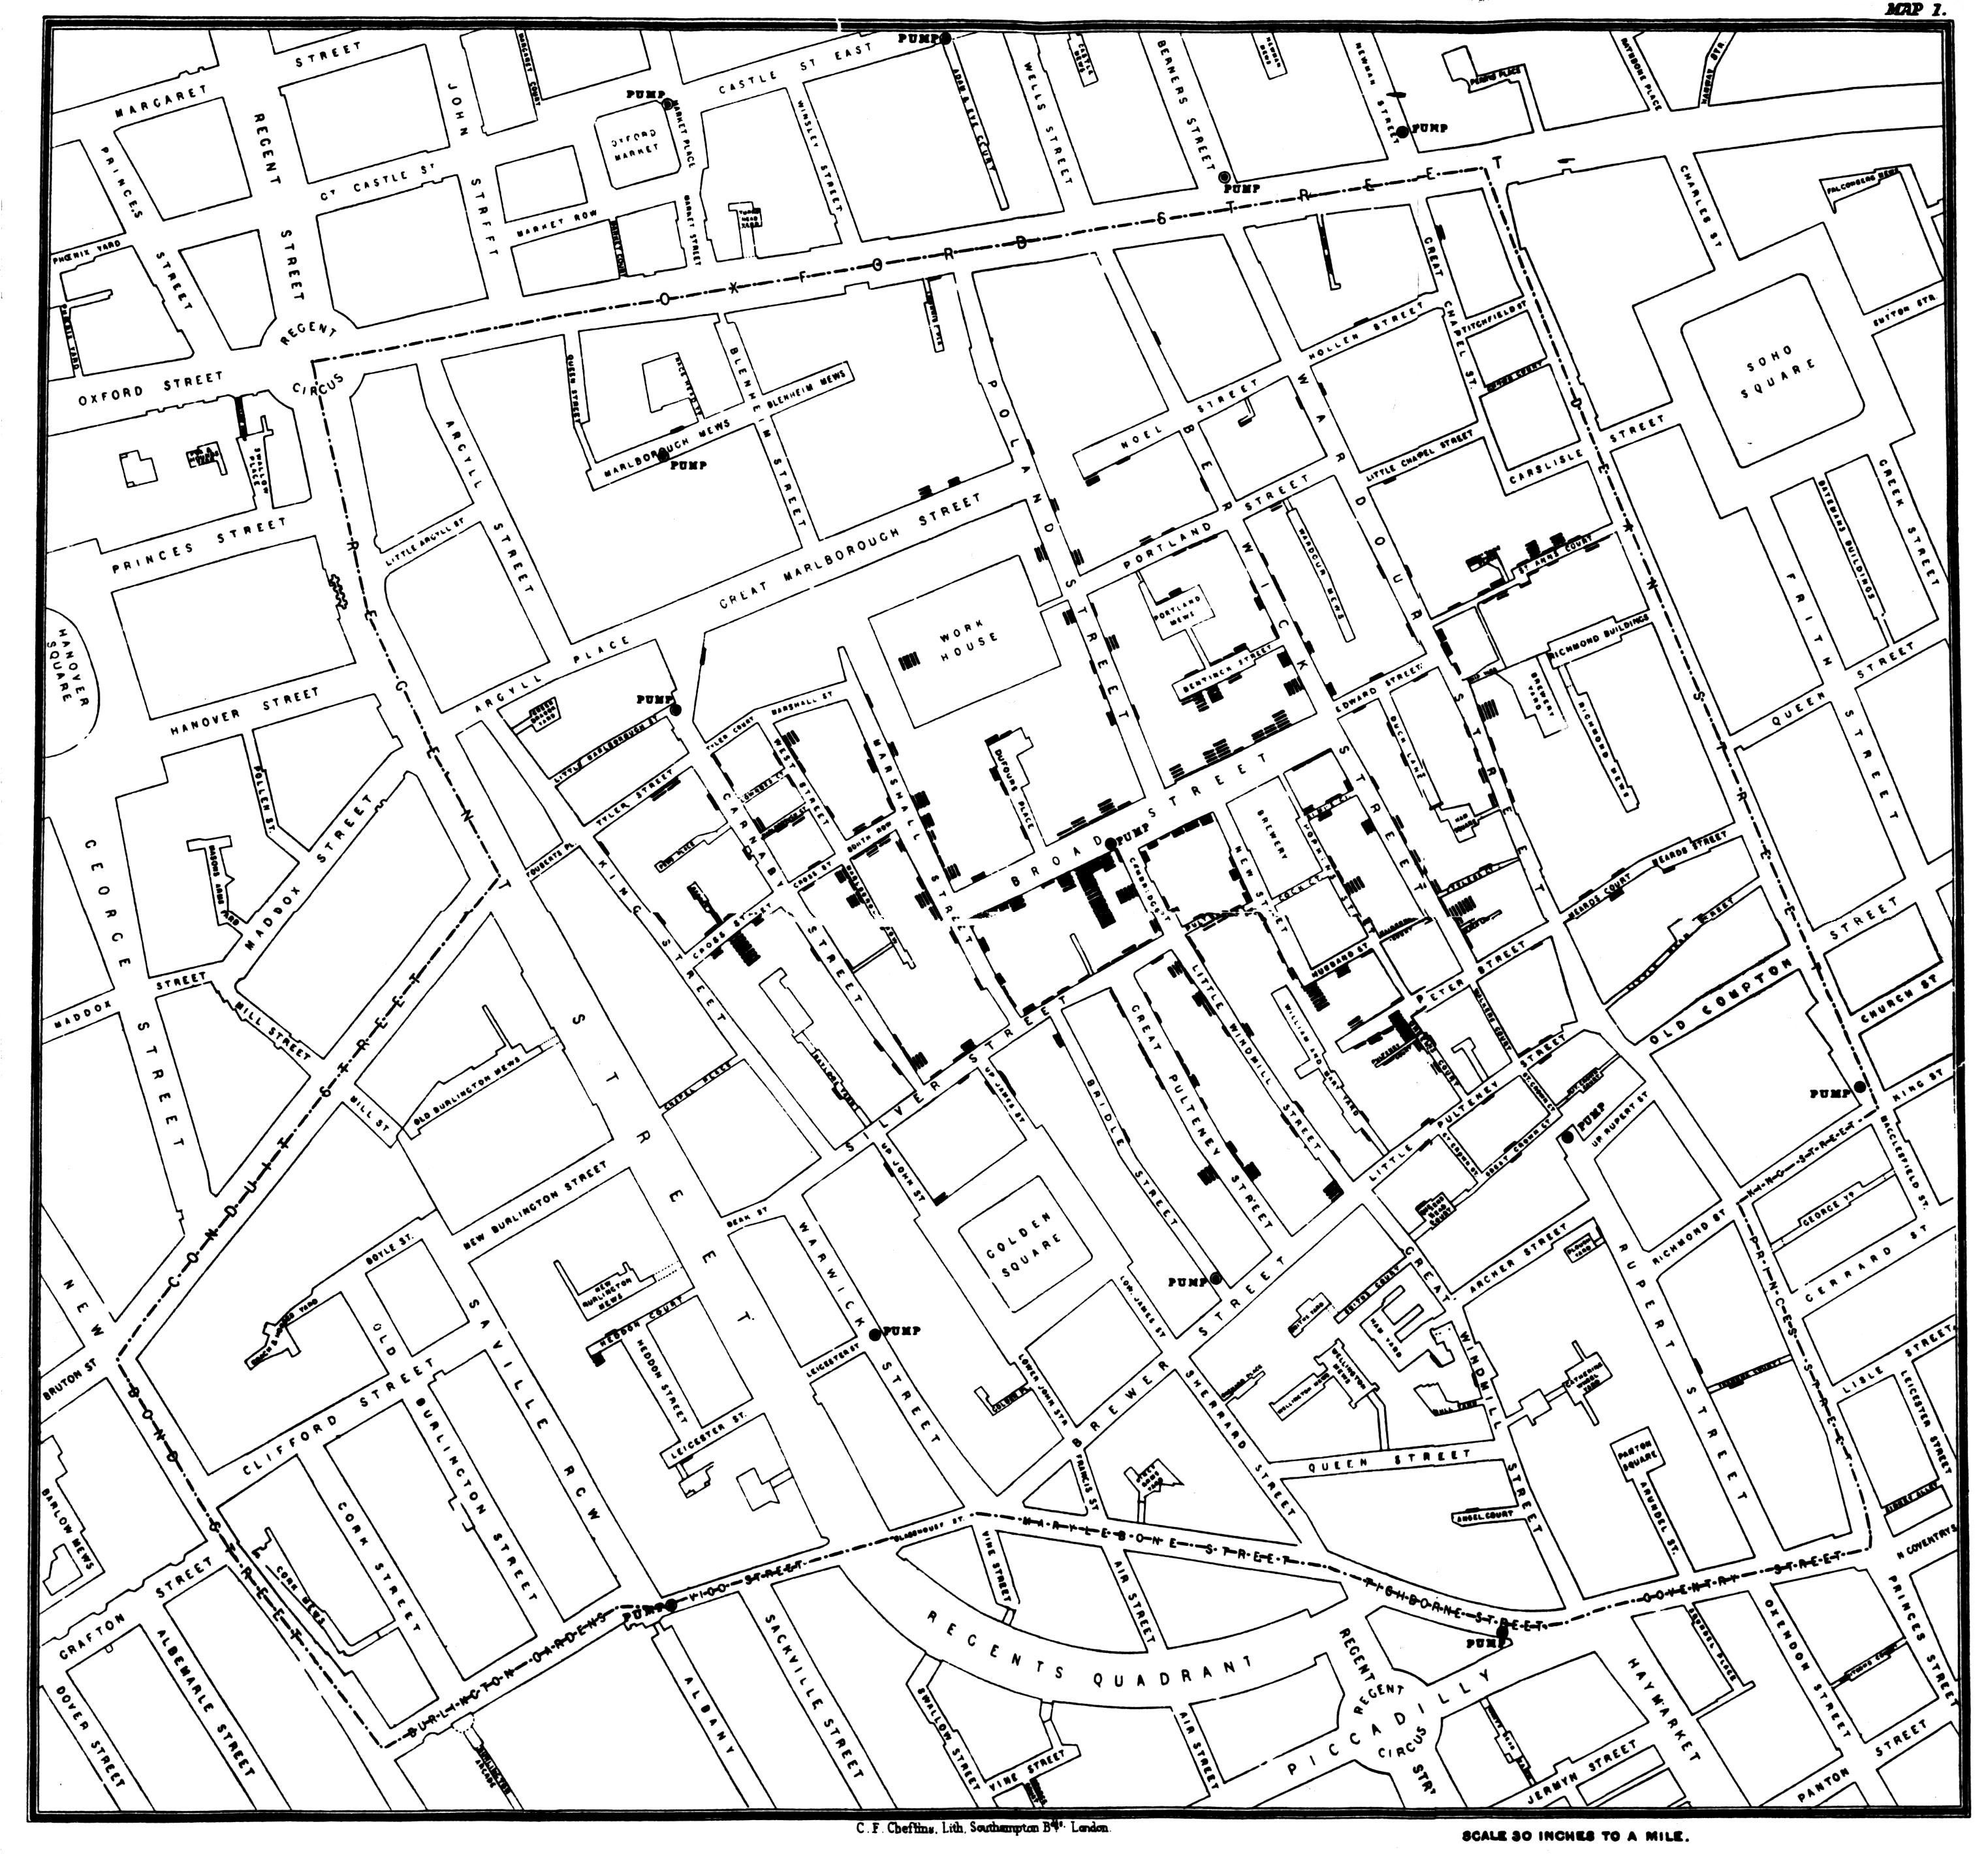
\includegraphics[width=\columnwidth]{Snow_cholera_map.jpg}
      \end{column}

      \begin{column}{.35\textwidth}
        \centering
        \caption{1854年英国Broad大街大规模爆发霍乱,流行病学家John
          Snow对此次霍乱进行了大量调研分析,并且发表了霍乱传播理论的论
          文,左图是其论文的主要依据:图中心东西
          方向的街道是Broad大街,黑点表示死亡地点\\
          这幅图形象揭示了一个重要现象,就是死亡地点都在街道中部一处水源
          (水井)周围,而市内其它水源周围极少发现死者,通过进一步调查他
          发现这些死者都饮用过这里的井水,从而发现了霍乱传播的源头是水
          井的把手,\emphText{这就是统计图形在公共卫生领域最早的应用}}
      \end{column}
    \end{columns}
  \end{figure}

\end{frame}

\begin{frame}{\subsecname}{霍乱传播之谜}

  \begin{figure}
    \begin{columns}
      \begin{column}{.6\textwidth}
        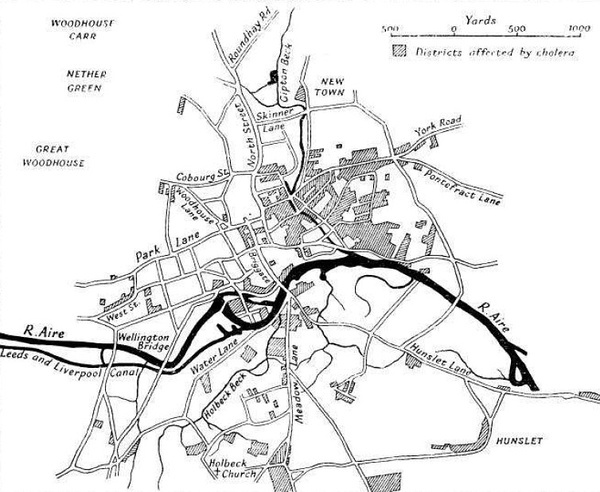
\includegraphics[width=\columnwidth]{Robert_Baker.jpg}
      \end{column}

      \begin{column}{.35\textwidth}
        \centering
        \caption{其实,在John Snow之前,有个叫Robert Baker的医生也研究
          了这个区域的霍乱问题,而且在1833年就绘制了左边这
          张霍乱的分布图。\\
          虽然Baker在这幅图中揭示了疾病和居住环境的联系:缺乏清洁用水和
          排水系统的居民点是疾病的高发区,\emphText{但是并没有显示发病
            率}。关于疾病起因的认知,他尽管方向正确但是并不完备,最终与
          伟大
          的发现擦肩而过\\
          \emphText{因此,只有充分完备的统计图形才能够真正应用于实践,
            这是一个漫长的科学过程}}
      \end{column}
    \end{columns}
  \end{figure}

\end{frame}

\begin{frame}{\subsecname}{切尔诺夫脸谱图(Chernoff Faces)}

  \begin{figure}
    \begin{columns}
      \begin{column}{.6\textwidth}
        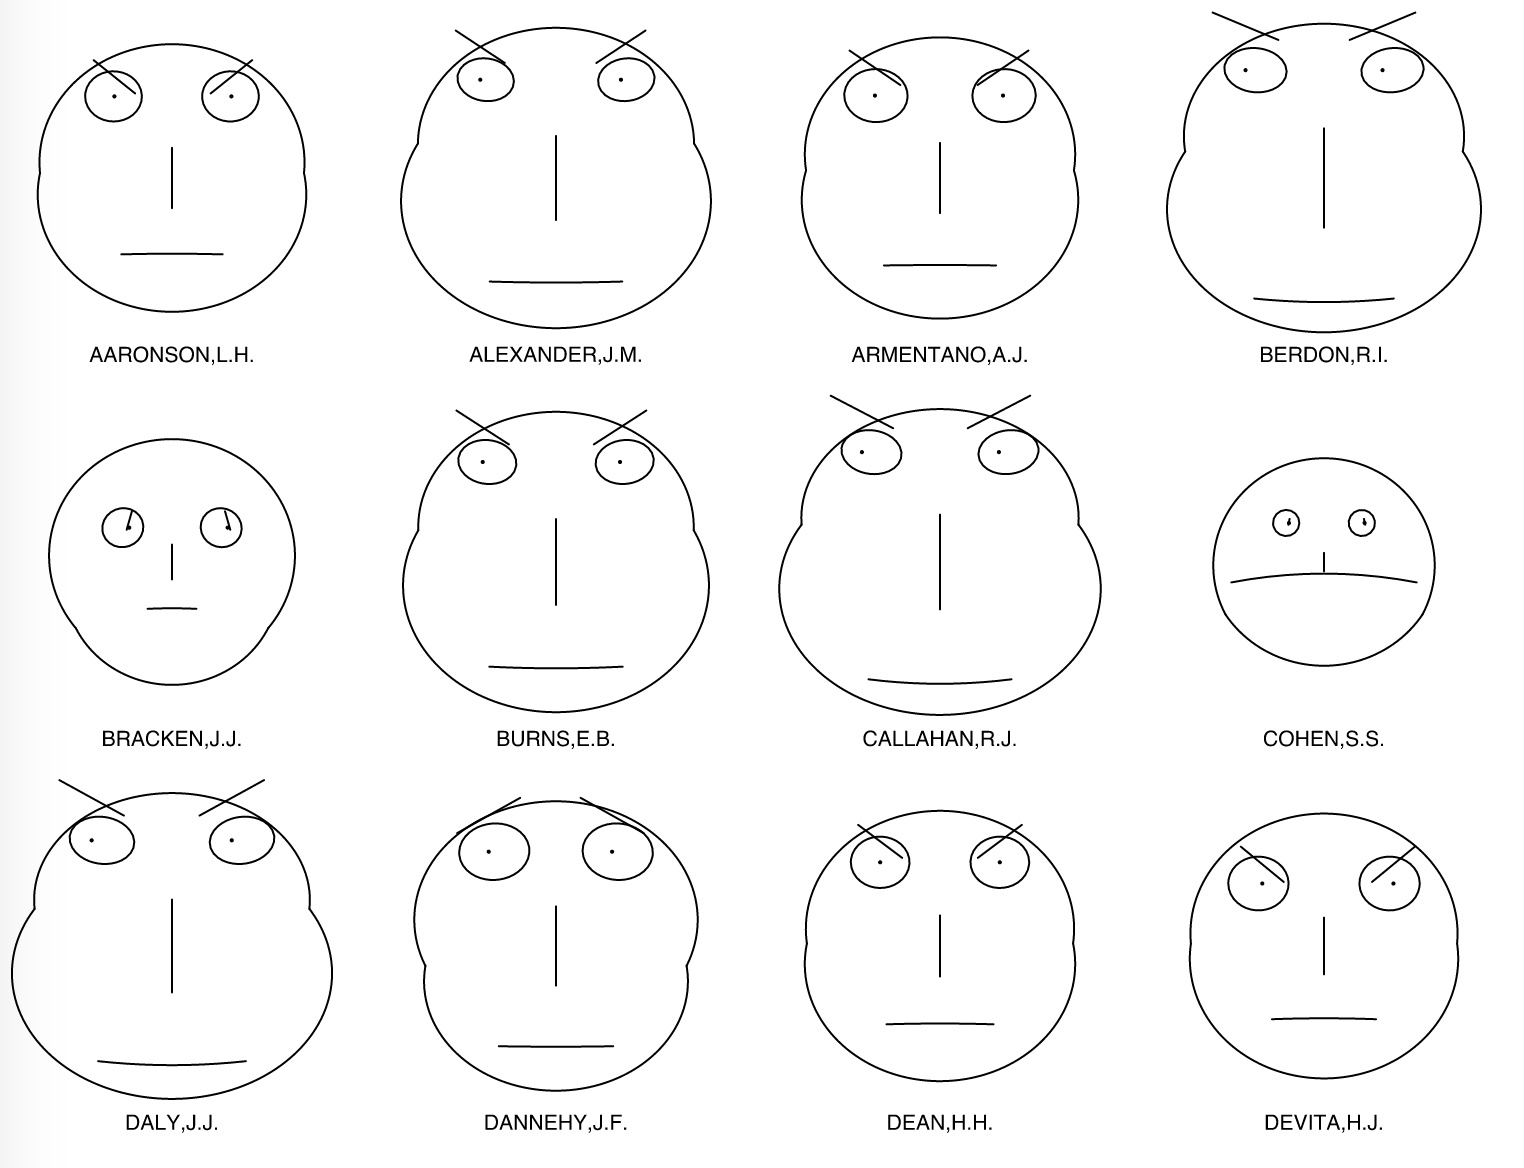
\includegraphics[width=\columnwidth]{切尔诺夫脸谱图.jpg}
      \end{column}

      \begin{column}{.35\textwidth}
        \centering
        \caption{切尔诺夫脸谱图(Herman Chernoff, 1973)\\
          这张很喜感的脸谱图其实是一种统计图,叫切尔诺夫脸谱图,是统计
          学家Herman Chernoff于1973年发明的,其基本思想是把多维数据的特
          征映射到卡通人脸中。由于人类非常善于识别脸部特征,脸谱化使得
          多维度数据容易被分析人员消化理解,有助于数据的规律和不规律性
          的可视化。\emphText{目前这种方法已被广泛应用于多地域经济战略
            指标数据分析,空间数据可视化等领域}}
      \end{column}
    \end{columns}
  \end{figure}

\end{frame}

%%%%%%%%%%%%%%%%%%%%%%%%%%%%%%%%%%%%%%%%%%%%%%%%%%%%%%%%%%%%
\section{统计绘图工具}
%%%%%%%%%%%%%%%%%%%%%%%%%%%%%%%%%%%%%%%%%%%%%%%%%%%%%%%%%%%%
\subsection{为什么要用绘图工具}
\begin{frame}{\subsecname}{}

  \begin{columns}
    \begin{column}{.5\textwidth}
      \begin{figure}
        \centering 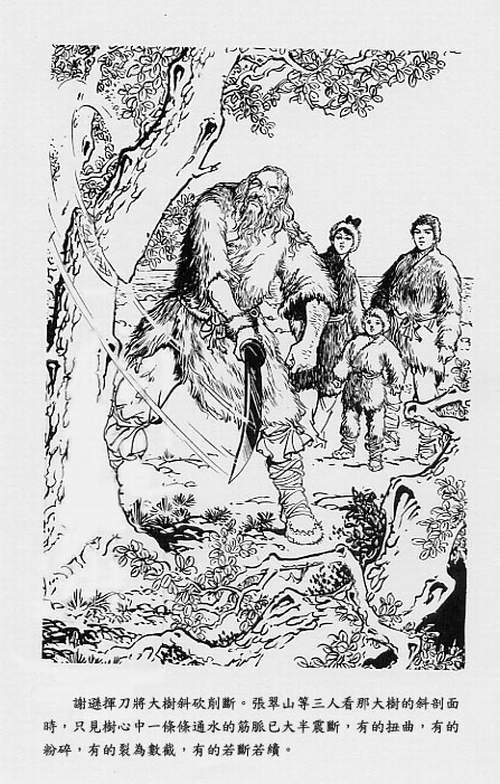
\includegraphics[width=0.9\columnwidth]{屠龙宝刀.jpg}
      \end{figure}
    \end{column}

    \begin{column}{.48\textwidth}
      \begin{ornamentblock}
        \centering
        {工欲善其事,必先利其器\\
          \rightline{\textemdash《论语·卫灵公》}}
      \end{ornamentblock}
      % \curlyframe{工欲善其事,必先利其器\\
      % \rightline{-----《论语·卫灵公》}}
    \end{column}
  \end{columns}

\end{frame}

\begin{frame}[c]{\subsecname}
  
  \begin{columns}
    \begin{column}{.6\textwidth}
      \begin{figure}
        \centering 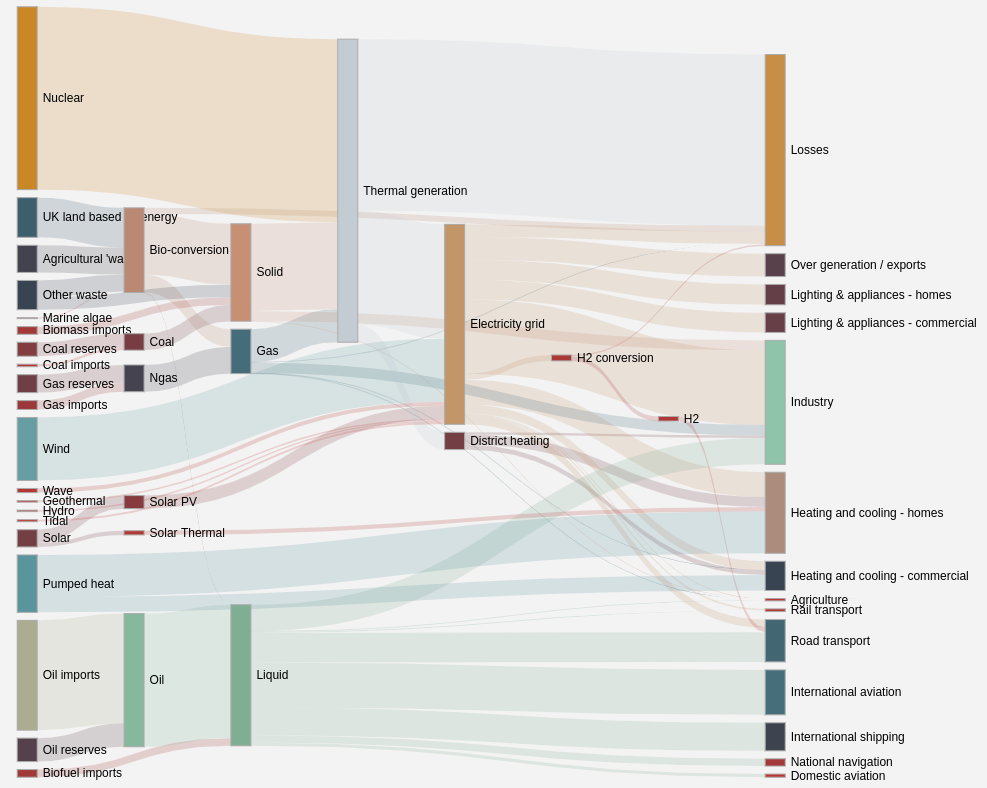
\includegraphics[width=\columnwidth]{sankey.png}
        \caption{看上去复杂但是直观的桑基图(Sankey diagram)}
      \end{figure}
    \end{column}

    \begin{column}{.4\textwidth}
      \begin{block}{直观与简单} \small
        \begin{itemize}
        \item[\HandRight] \emphText{统计量是统计图形最关键的构成因素},
        因此,优秀的统计图形背后必然隐藏着重要的统计量
        \item[\HandRight] 图形的首要作用是“直观”展示统计量信息,
        但是\emphText{能够直观理解的信息未必是“简单”的}
        \item[\HandRight] 使用合适的工具可以让信息的表达既“直观”又“简单” 
        \end{itemize}
      \end{block}
    \end{column}
  \end{columns}
    
\end{frame}

\subsection{何为利器}
\begin{frame}[t]{\subsecname}
  \begin{itemize}
    \hilite<1> \item 统计计算功能齐全
    \hilite<2> \item 图形元素易于控制
    \hilite<3> \item 统计图形类型种类丰富
  \end{itemize}

\begin{figure}[ht]
  \centering 
\includegraphics[width=0.8\textwidth]{stat_tools.png}
  \caption{常见的一些统计绘图工具}
\end{figure}

\end{frame}

\subsection{所见即所得工具}

\begin{frame}[t]{\subsecname}{excel}
  \begin{itemize}
    \hilite<1> \item 微软公司开发的电子数据表软件,从1985年发布1.0版本
    至今已经30多年历史,是电子数据表类软件的工业标准\hilite<2> \item 优
    秀的人机交互设计,所见即所得\hilite<3> \item 能够完成简单的统计功能
    以及数据绘图,但并不是统计软件
  \end{itemize}

\begin{overlayarea}  {\textwidth}{\textheight} 
  \only<1>{
    \begin{figure}\centering
      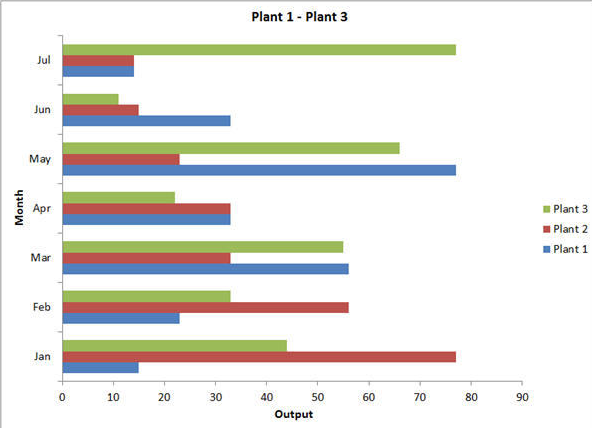
\includegraphics[width=0.65\columnwidth] {excel条形图.png}
      %{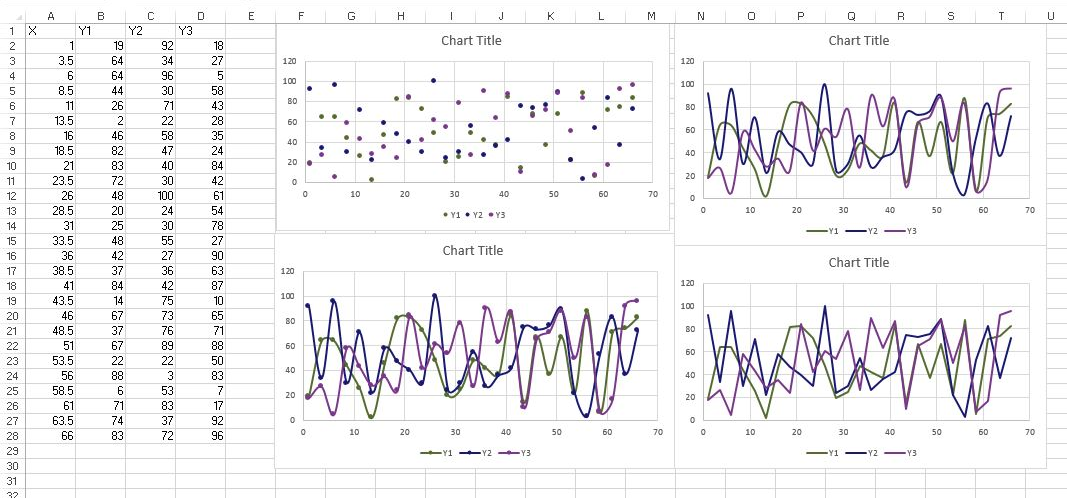
\includegraphics[width=0.45\columnwidth] {excel折线图.png}}
      \caption{表示绝对数值大小的条形图}
    \end{figure}}

  \only<2>{
    \begin{figure}\centering
      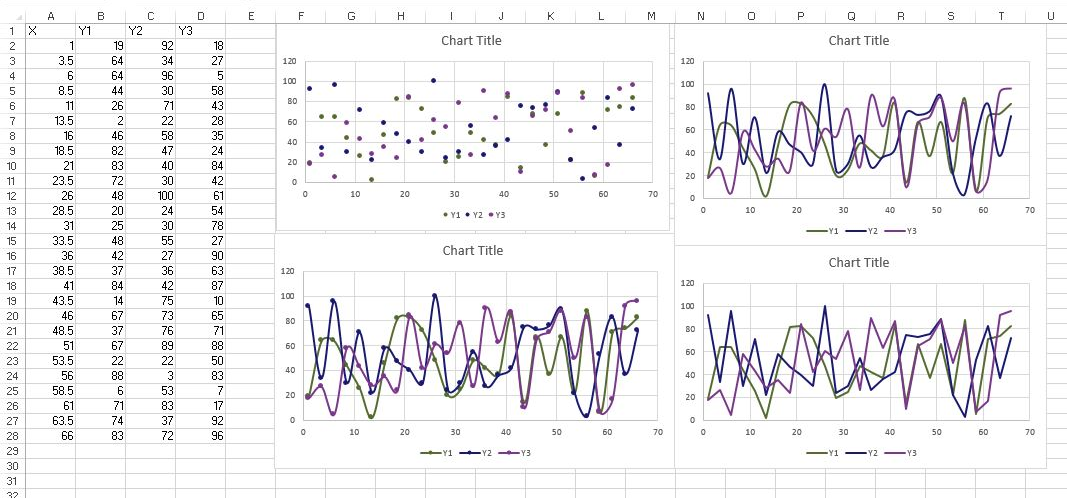
\includegraphics[width=\columnwidth] {excel折线图.png}
      \caption{表示绝对数值大小的折线图}
    \end{figure}}
  
  \only<3>{
    \begin{figure}[ht]
      \centering 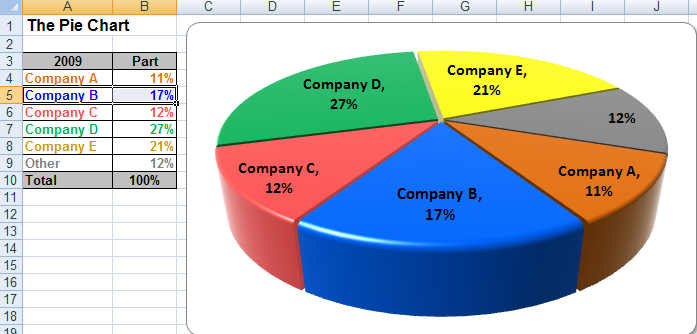
\includegraphics[width=\columnwidth]{excel饼图.png}
      \caption{表示比例大小的饼图}
    \end{figure}}

  \only<4>{
    \begin{figure}[ht]
      \centering 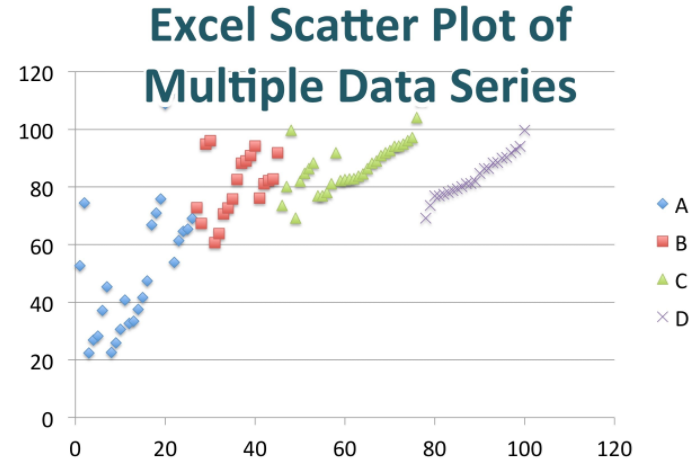
\includegraphics[width=0.7\columnwidth]{excel散点图.png}
      \caption{表示二维变量关系的散点图}
    \end{figure}}
   
  \only<5->{
    \begin{alertblock}{excel作为统计绘图工具的缺点}
      \begin{itemize} \small
        \hilite<5> \item[\PencilLeftDown] excel擅长对原始数据的展示,统
        计分析和建模功能十分有限。因此,著名统计学家Leland
        Wilkinson\footnote[frame,1]{统计学经典书籍《The Grammar of
          Graphics》一书的作者,任职SPSS公司十年,而且一直领导其可视化
          小组}说\emphTextStep{5-}{“给统计刊物投稿时永远不要用Excel作图”}
        \hilite<6> \item[\PencilLeftDown] 数据量的限制,处理速度慢
        \hilite<7> \item[\PencilLeftDown] 只能在windows单机上运行,无
          法开展跨平台和分布式计算,不具备大规模数据管理功能
        %\hilite<8> \item[\PencilLeftDown] 商业软件,价格不菲
      \end{itemize}
    \end{alertblock}}
\end{overlayarea}  
\end{frame}

\begin{frame}[t]{\subsecname}{SPSS}
  \begin{itemize}
    \hilite<1> \item 易学易用的统计分析软件
    \hilite<2> \item 功能全面的统计分析软件
    \hilite<3> \item 界面友好
  \end{itemize}

\begin{overlayarea}  {\textwidth}{\textheight}
  \only<1-3>{
    \begin{figure}[ht]
      \centering 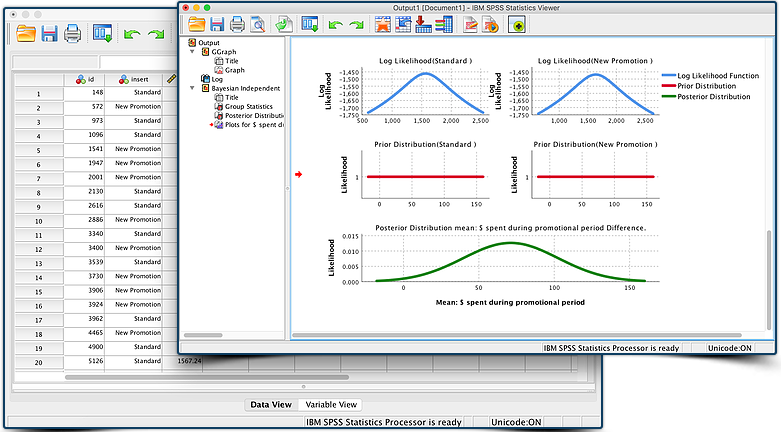
\includegraphics[width=0.9\textwidth]{SPSS.png}
      \caption{SPSS用户操作界面}
    \end{figure}}
   
  \only<4->{
    \begin{alertblock}{SPSS及其他所见即所得工具的缺陷}
      \begin{itemize} \small
        \hilite<4> \item[\PencilLeftDown] 按钮的数量总是有限的,而统计模型是无限的
        \hilite<5> \item[\PencilLeftDown] 计算机完成了太多
        本该由用户完成的图形要素控制
        \hilite<6> \item[\PencilLeftDown] 生成一张图易,生成N张图难
        \hilite<7> \item[\PencilLeftDown] 贫穷限制了想象力,模块单独付费
      \end{itemize}
    \end{alertblock}}
\end{overlayarea}
\end{frame}

\subsection{所想即所得工具}
\begin{frame}[t]{\subsecname}{SAS}
  \begin{itemize}
    \hilite<1> \item 1960年诞生于SAS软件研究所,老牌专业统计软件
    \hilite<2> \item 基于数据库进行数据管理,具有大型数据集处理分析能力
    \hilite<3> \item 有专门的SAS认证考试,包括程序员、业务分析师、数据挖掘、系统开发
           专家和系统管理专家五种不同角色
  \end{itemize}
  
  \begin{overlayarea} {\textwidth}{\textheight}
    \only<1-4>{
      \begin{figure}
        \centering 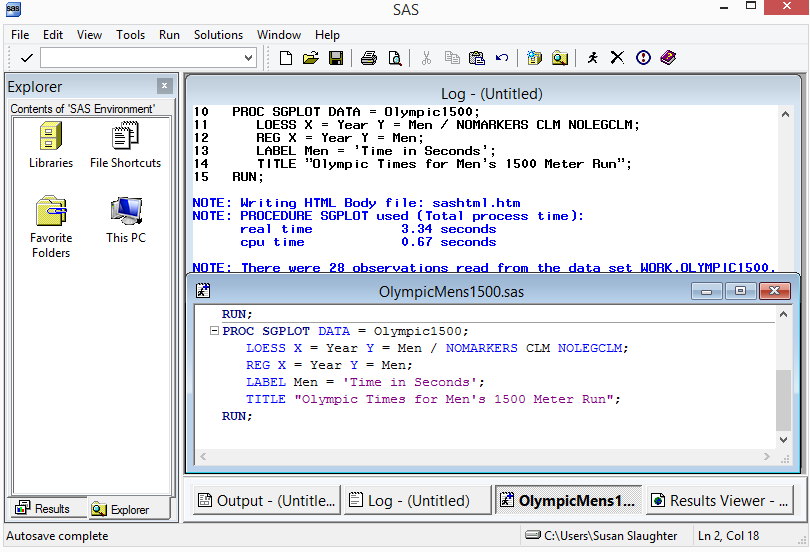
\includegraphics[width=0.7\columnwidth]{sas_ui.png}
        \caption{SAS软件界面}
      \end{figure}}
  \end{overlayarea}
\end{frame}

\begin{frame}[t, fragile]{\subsecname}{SAS}
  \begin{itemize}
    \item 200多个集成模块,涵盖了主流统计模型和分析方法,而且通过内置
           脚本语言实现统计建模和绘图等功能
  \end{itemize}
 
      \begin{columns}
        \begin{column}{.5\textwidth}
          \begin{figure}
            \centering
            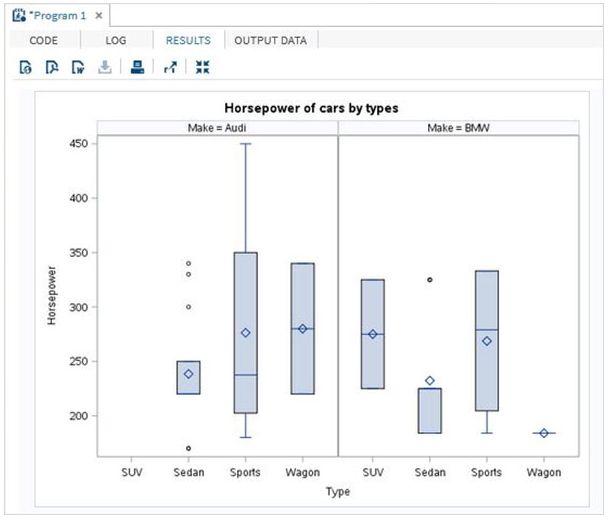
\includegraphics[width=0.8\columnwidth]{sas_boxplot.png}
            \caption{箱形图(Box plot)}
          \end{figure}
        \end{column}

        \begin{column}{.5\textwidth}
\begin{lstlisting}[language=SAS]
PROC SQL;
create table CARS1 as
SELECT make,model,type,invoice,horsepower,length,weight
 FROM SASHELP.CARS
WHERE make in ('Audi','BMW');
RUN;

PROC SGPLOT  DATA=CARS1;
  VBOX horsepower 
  / category = type;

   title 'Horsepower of cars by types';
RUN; 
\end{lstlisting}
        \end{column}
      \end{columns}
\end{frame}

\begin{frame}[t]{\subsecname}{S-Plus}
    \begin{itemize}
      \item S语言是1976年AT\&T贝尔实验室开发的一种用于统计计算的解释型编程语言
    \end{itemize}

    \begin{figure}
      \centering 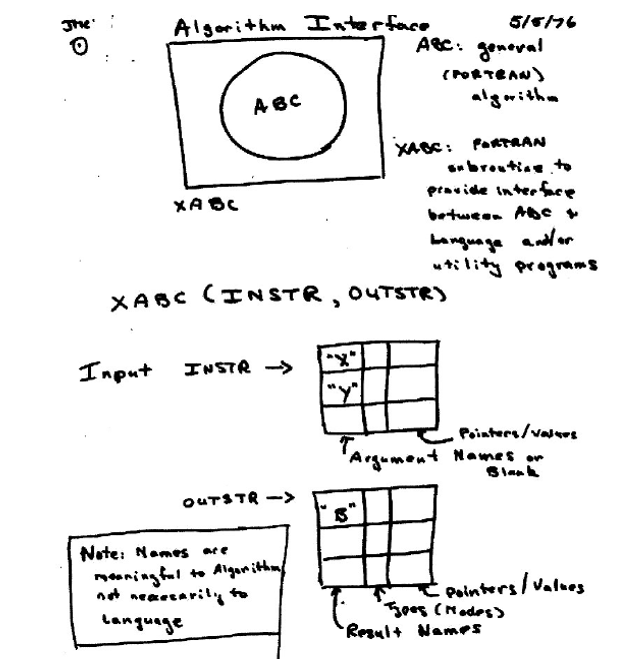
\includegraphics[width=0.5\columnwidth]{S_init.png}
      \caption{S语言的设计草图(1976.5.5)}
    \end{figure}

\end{frame}   

\begin{frame}[t, fragile]{\subsecname}{S-Plus}
    \begin{itemize}
      \item 与SAS内置脚本语言相比,S语言更加符合现代程序语言的设计,方便灵活控制
            图形输出,制作既精美又专业的统计图形
      \item 能够与其他主流程序语言集成
    \end{itemize}

    \begin{onlyenv}<1>
      \begin{columns}
        \begin{column}{.7\textwidth}
          \begin{figure}
            \centering
            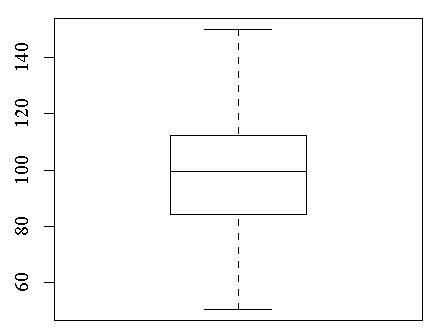
\includegraphics[width=0.8\columnwidth]{splus_boxplot.png}
            \caption{箱形图(Box plot)}
          \end{figure}
        \end{column}

        \begin{column}{.3\textwidth}
\begin{lstlisting}[language=S]
  boxplot(Weight)
\end{lstlisting}
        \end{column}
      \end{columns}
    \end{onlyenv}
\end{frame}    

\begin{frame}[t]{\subsecname}{S-Plus}
    \begin{itemize}
      \item S-Plus是基于S语言开发的商业化统计软件,1993年由MathSoft公司开发,
            2008年起由TIBCO负责运维
      \item 与SPSS和SAS并称世界三大统计软件,具有专业的统计功能
    \end{itemize}

    \begin{figure}
      \centering 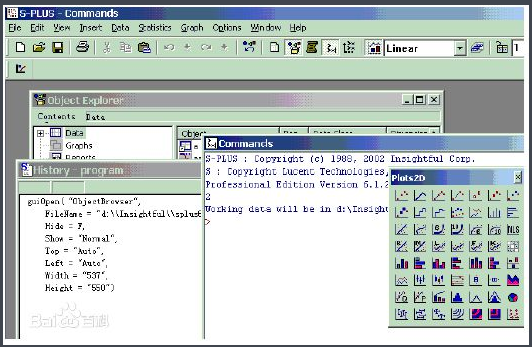
\includegraphics[width=0.8\columnwidth]{splus_ui.png}
      \caption{S-Plus软件界面}
    \end{figure}
\end{frame}    

\begin{frame}{\subsecname}{}
  % \begin{variableblock}{所想即所得工具}{bg=green!20,fg=black}{fg=white,bg=SpringGreen4}
  %   \begin{itemize}
  %   \item wowo
  %   \item sdsfs
  %   \end{itemize}
  % \end{variableblock}
\onslide<1->{
  \begin{goodbox}{所想即所得工具的优势}
     \begin{itemize}
     \item[\PencilLeftDown] 想象力有多大,世界就有多精彩
     \item[\PencilLeftDown] 花有重开日,人无再少年
     \item[\PencilLeftDown] 深入算法内核,由术至道 
     \end{itemize}
  \end{goodbox}}

\onslide<2->{
  \begin{badbox}{所想即所得工具的劣势}
     \begin{itemize}
     \item[\PencilLeftDown] 人机交互全靠命令,需要一定的编程基础
     \item[\PencilLeftDown] 需要扎实的统计学基础,学习曲线陡峭
     \item[\PencilLeftDown] 键盘易损坏,手指易抽筋    
     \end{itemize}
  \end{badbox}}

\end{frame} 

%%%%%%%%%%%%%%%%%%%%%%%%%%%%%%%%%%%%%%%%%%%%%%%%%%%%%%%%%%%
\section{R简介}
%%%%%%%%%%%%%%%%%%%%%%%%%%%%%%%%%%%%%%%%%%%%%%%%%%%%%%%%%%%%
\subsection{为什么用R}
\begin{frame}{\subsecname}{}

  \begin{columns}
    \begin{column}{.5\textwidth}
      \begin{figure}
        \centering 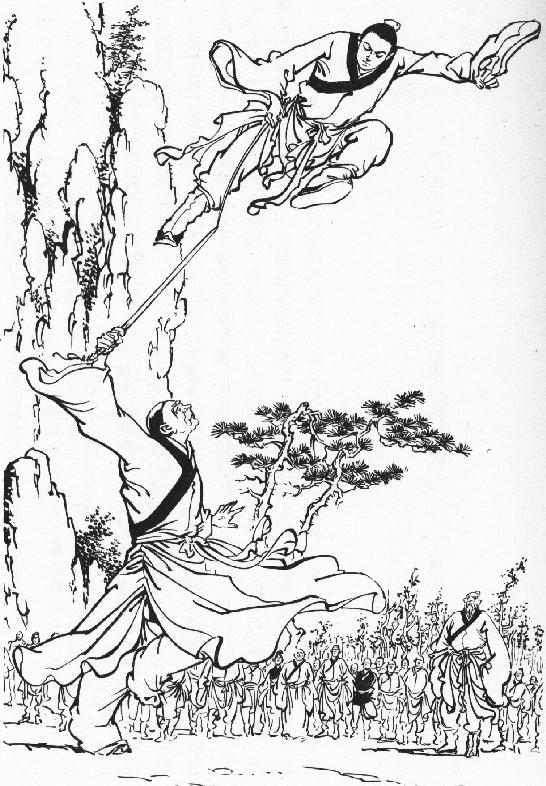
\includegraphics[width=0.9\columnwidth]{乾坤大挪移.jpg}
      \end{figure}
    \end{column}

    \begin{column}{.48\textwidth}
      \begin{ornamentblock}
        \centering
        {君子性非异也,善假于物也\\
          \rightline{\textemdash《荀子·劝学》}}
      \end{ornamentblock}
      % \curlyframe{工欲善其事,必先利其器\\
      % \rightline{-----《论语·卫灵公》}}
    \end{column}
  \end{columns}
\end{frame}

\begin{frame}[t]{\subsecname}{R的历史}

\begin{itemize}
\hilite<1> \item R诞生于1995年,由新西兰Auckland大学统计学家\emphText{R}obert Gentleman
        和\emphText{R}oss Ihaka开发,而且完全开放源代码,是一款
        基于GNU General Public License(GPL)协议的开源软件
\hilite<2> \item R是“所想即所得”工具,其核心是基于S语言设计的R语言,S语言的代码可以不经过
        任何修改就在R中运行,因此R被看做是S语言的非商业化实现
\hilite<3> \item 由于两位开发者的名字都以“R”开头,而且为了向S语言致敬,因此命名为R 
\end{itemize}

\begin{overlayarea} {\textwidth}{\textheight}
    \begin{figure}\centering
      \captionsetup[subfigure]{labelformat=empty} 
      \subfloat[Ross Ihaka]
      {
\includegraphics[width=0.45\columnwidth]{Ross_Ihaka.png}} \vspace{1pt}
      \subfloat[Robert Gentleman]
      {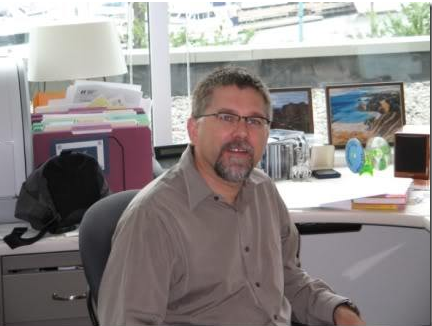
\includegraphics[width=0.4\columnwidth]{Robert_Gentleman.png}} 
    \end{figure}
\end{overlayarea}

\end{frame}

\begin{frame}[t]{\subsecname}{R的优势}
\begin{itemize}
\hilite<1> \item R具备S-Plus几乎所有的优点,而且更加小巧轻便
\hilite<2> \item 开源项目,完全免费,这点是其他统计软件都不具备的
\hilite<3> \item 世界各地有大量研究机构和专业统计人员使用
                 并自愿贡献代码,具有良好的生态系统
\end{itemize}  

\begin{overlayarea}{\textwidth}{\textheight}

\only<1-2>{
  \begin{figure}[ht]
    \centering
    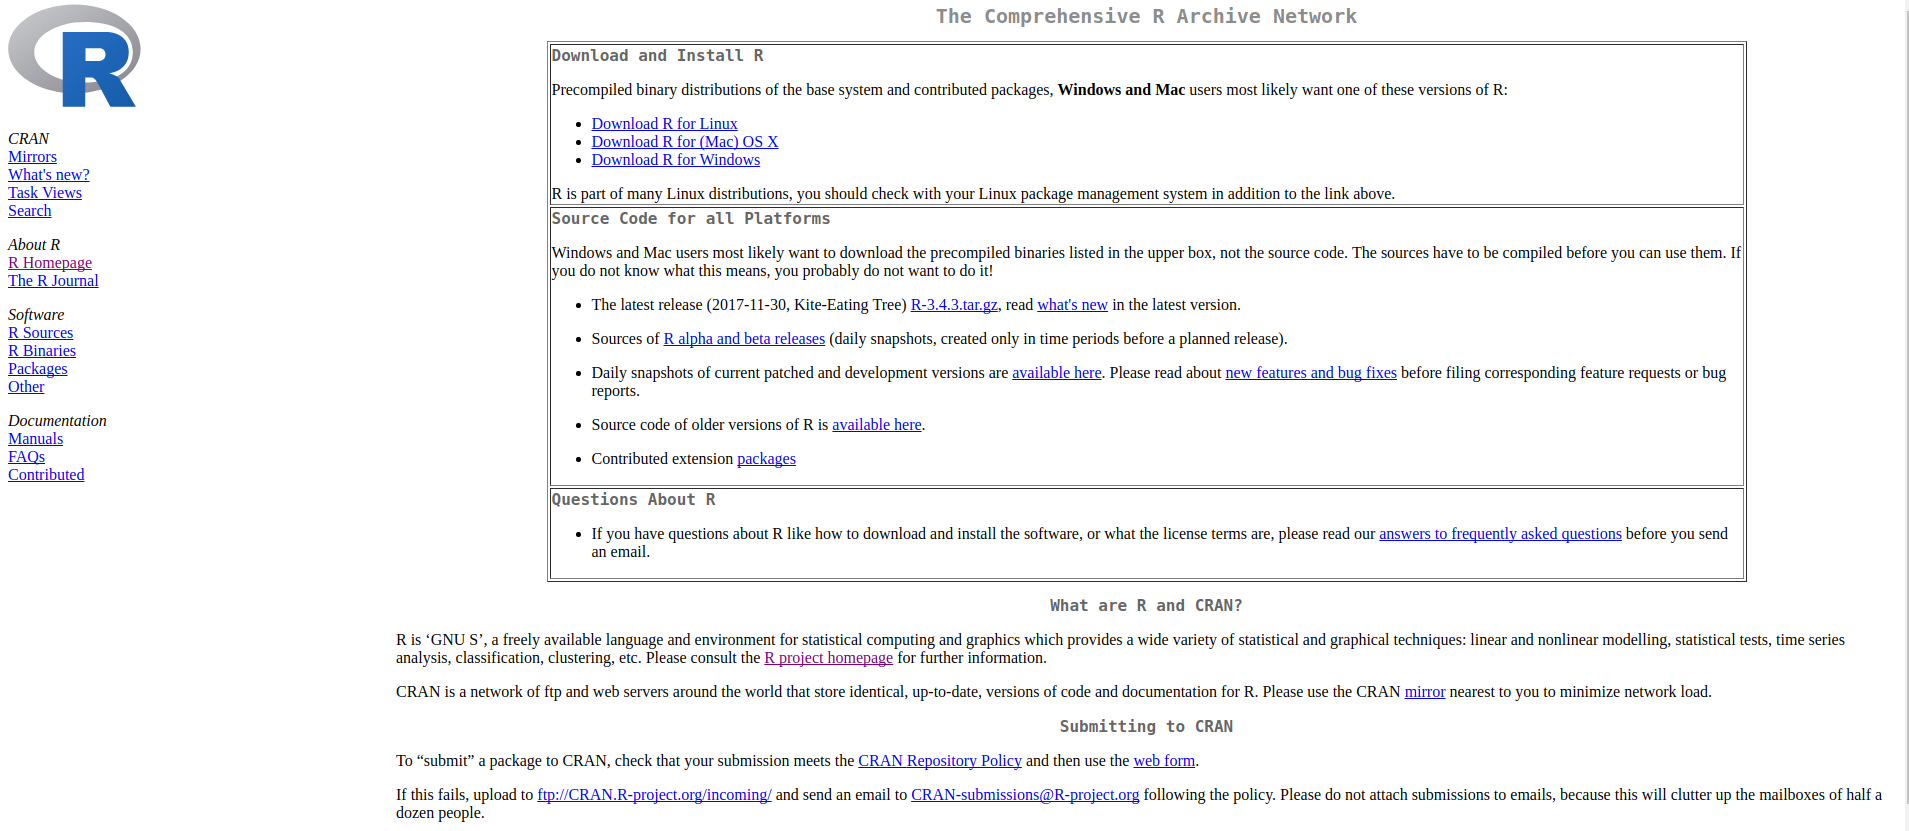
\includegraphics[width=\columnwidth]{CRAN.png}
    \caption{R的官方网站CRAN(https://cran.r-project.org/)}
  \end{figure}}

\only<3>{
  \begin{figure}[ht]
    \centering
    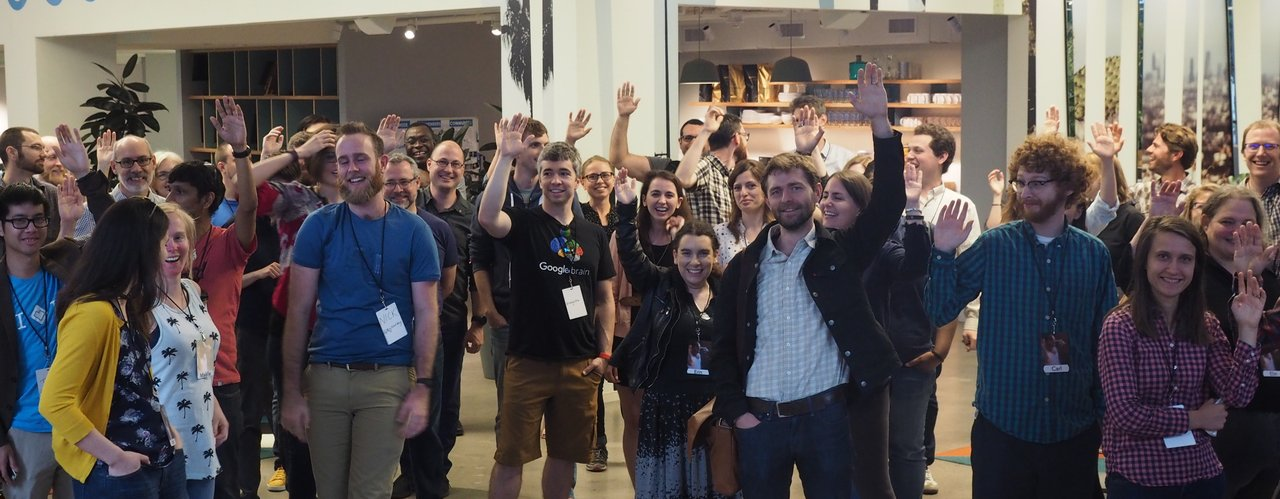
\includegraphics[width=\columnwidth]{R_community.jpg}
    \caption{来自世界各地R的无私贡献者们}
  \end{figure}}
\end{overlayarea}

\end{frame} 

\begin{frame}[t]{\subsecname}{R的优势}
\begin{itemize}
\hilite<1> \item R是高度模块化软件,通过各种程序包(package)来扩展其功能,目前CRAN上
                 接收的程序包超过12000个,绝大多数来自自愿者的贡献
\hilite<2> \item 与其他语言具有极好的兼容性
\hilite<3-> \item 目前最新的统计模型和算法几乎都有R的实现版本,与统计研究前沿相接轨 
\end{itemize}  

\begin{overlayarea}{\textwidth}{\textheight}
\only<1>{
  \begin{figure}[ht]
    \centering
    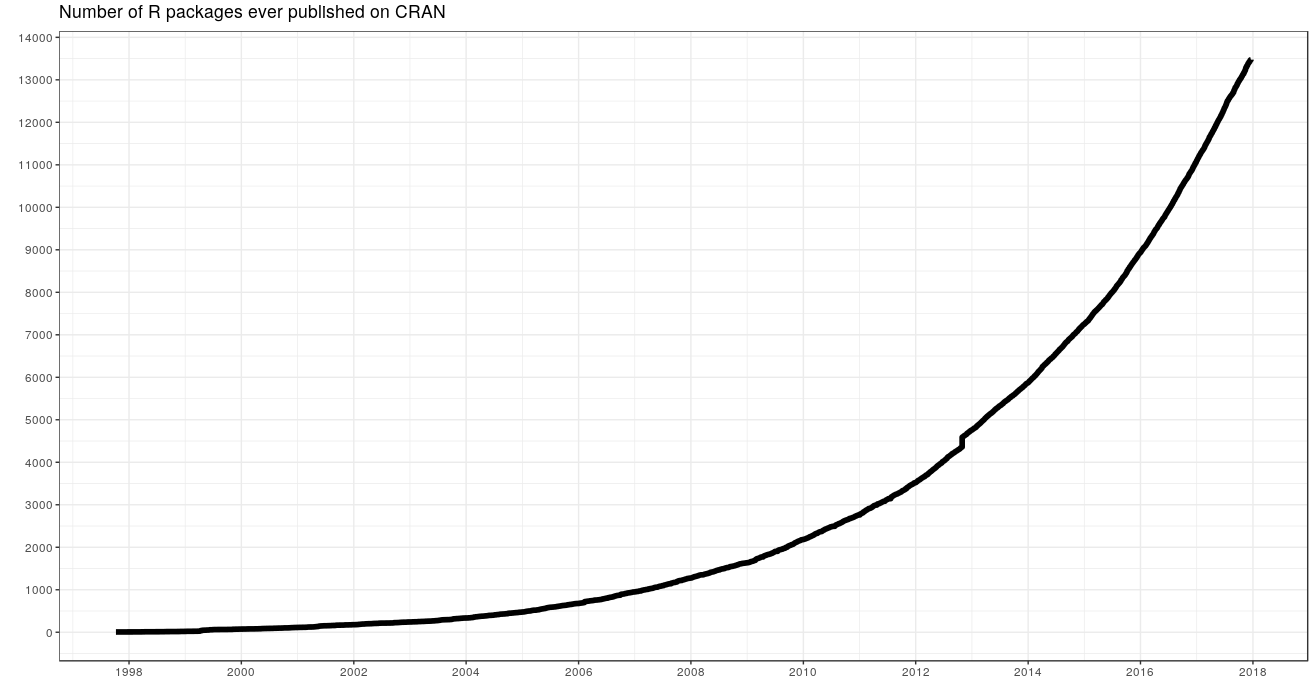
\includegraphics[width=0.8\columnwidth]{number_of_R_packages.png}
    \caption{历年R packages提交的数量统计}
  \end{figure}}

\only<2>{
\begin{block}{R语言的兼容性}
  \begin{itemize}
  \item[\PencilLeftDown] \emphText{内部兼容}:由于R语言本身是解释性语言,
    执行效率较低,因此R的底层函数有很大一部分代码是C语言和Fortran语言编
    写的
  \item[\PencilLeftDown] \emphText{外部兼容}:目前主流的编程语言,例
    如JAVA、c++、python等几乎都有相应的程序库来调用R语言编写的程序,来
    帮助这些编程语言简化统计计算和绘图相关的功能
  \end{itemize}
\end{block}}

\only<3>{
  \begin{figure}[ht]
    \centering
    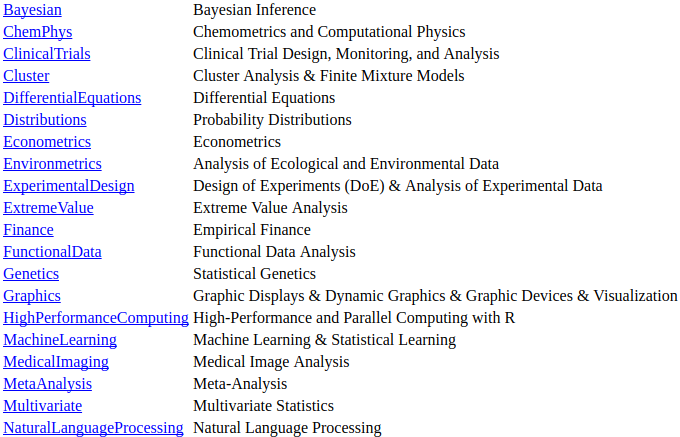
\includegraphics[width=0.6\columnwidth]{CRAN_TASK1.png}
    \caption{R packages的任务分类}
  \end{figure}}

\only<4>{
  \begin{figure}[ht]
    \centering
    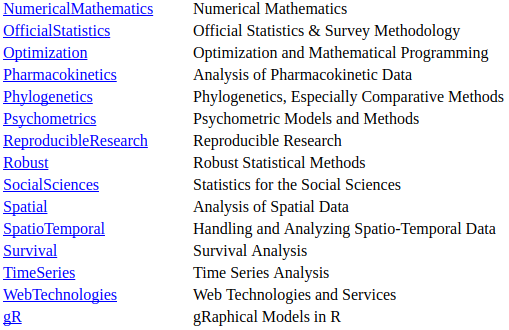
\includegraphics[width=0.6\columnwidth]{CRAN_TASK2.png}
    \caption{R packages的任务分类}
  \end{figure}}
\end{overlayarea}

\end{frame} 

\subsection{基础知识}
\begin{frame}[shrink]{\subsecname}{R的工作原理}
\begin{itemize}
\item 在R中进行的所有操作都是针对存储在\emphText{内存中的对象}
\item 用户通过输入命令调用函数,\emphText{分析结果可以被直接显示在屏幕上,也可以被存入某个对象或被
写入硬盘}(如图片对象)
\item 因为分析结果本身也是对象,所以它们也能\emphText{被视为数据并能像一般数据那样被处理分析}
\item 数据可以从本地磁盘读取,也可从远程服务器端获得 
\end{itemize} 

\begin{figure}[ht]
  \centering
  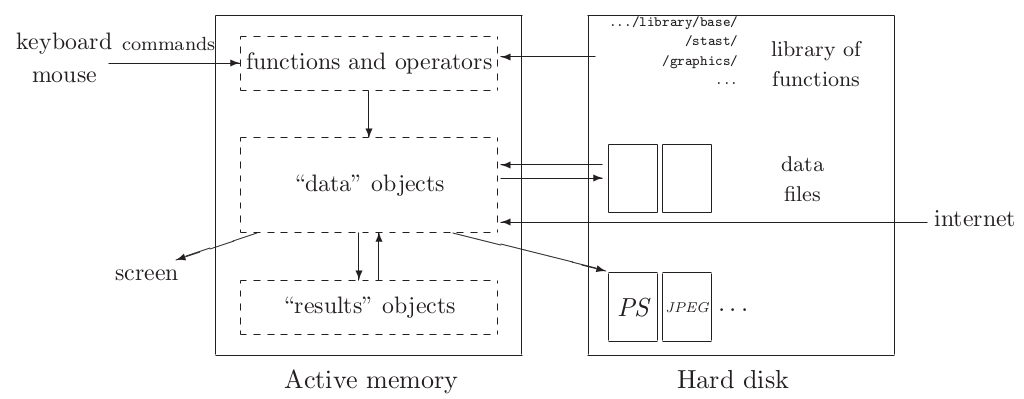
\includegraphics[width=0.9\columnwidth]{R_principle.png}
  \caption{R的工作原理}
\end{figure}
\end{frame}

\begin{frame}[t]{\subsecname}{安装运行环境}
\begin{itemize}
\hilite<1> \item R的主安装程序由自愿者进行编译上传,基本上每个在CRAN上可以自由下载,包括windows、linux
                 和mac三大主流平台
\hilite<2>\item 安装后的程序界面是一个交互式命令行终端,默认由一个“>”符号表示命令输入和结果
                 输出指示符
\hilite<3-> \item 在windows有一个简陋的GUI,linux和mac下默认只有CLI终端 
\end{itemize} 

\begin{overlayarea}{\textwidth}{\textheight}
\only<1>{
  \begin{figure}[ht]
    \centering
    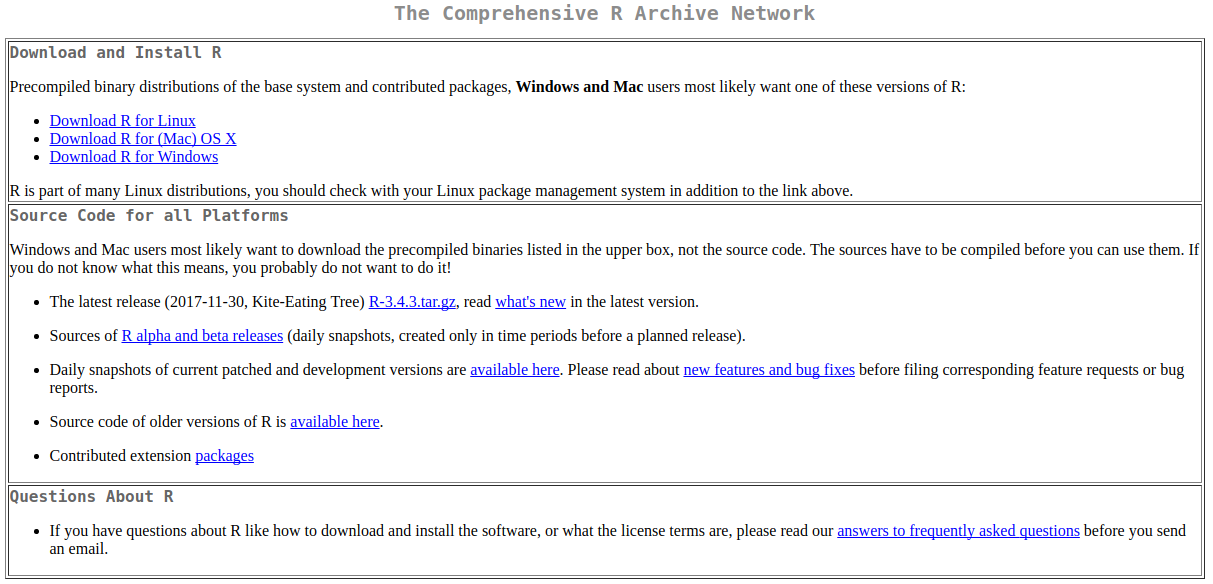
\includegraphics[width=0.8\columnwidth]{R_download.png}
    \caption{R在CRAN的下载界面}
  \end{figure}}

\only<3>{
  \begin{figure}[ht]
    \centering
    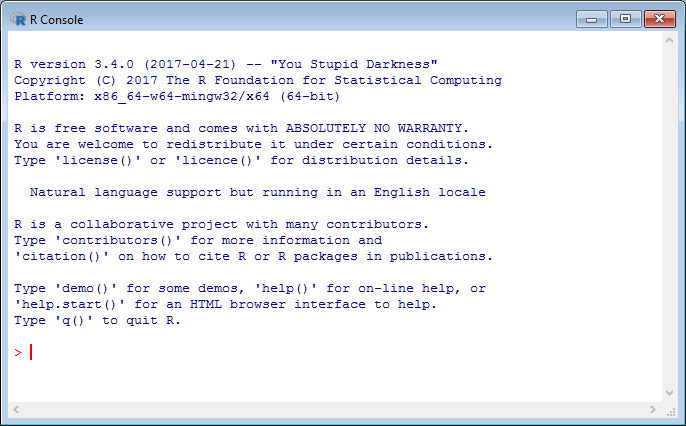
\includegraphics[width=0.6\columnwidth]{R_gui.png}
    \caption{R在windows下的GUI}
  \end{figure}}

\only<4>{
  \begin{figure}[ht]
    \centering
    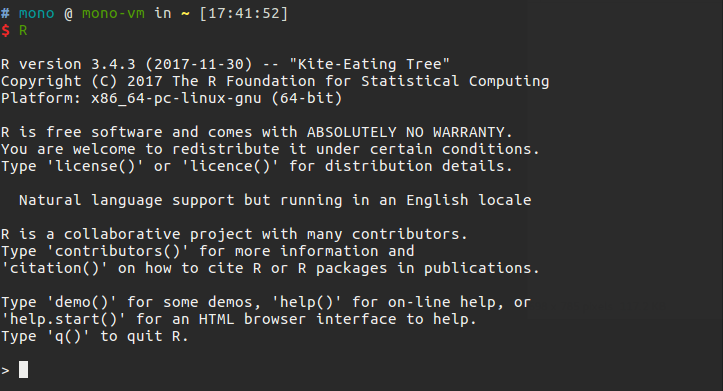
\includegraphics[width=0.7\columnwidth]{R_cli.png}
    \caption{R在linux下的cli终端}
  \end{figure}}
\end{overlayarea}
\end{frame}

\begin{frame}[t, fragile]{\subsecname}{基本操作}
\begin{itemize}
  \item R的第一种操作就是\emphText{“输入命令$\rightarrow$回车$\rightarrow$输出结果”}这种
             标准的交互式命令行方式  
\end{itemize} 

\begin{overlayarea}{\textwidth}{\textheight}
\begin{onlyenv}<1>
\begin{rcode}
> x = runif(100); y = 0.2*x + 0.1*rnorm(100)
> fit = lm(y ~ x)
> summary(fit)

Call:
lm(formula = y ~ x)

Residuals:
     Min       1Q   Median       3Q      Max 
-0.30665 -0.05002 -0.01135  0.06047  0.24599 

Coefficients:
            Estimate Std. Error t value Pr(>|t|)    
(Intercept)  0.02052    0.01670   1.229    0.222    
x            0.17510    0.03107   5.636 1.67e-07 ***
---
Signif. codes:  0 ‘***’ 0.001 ‘**’ 0.01 ‘*’ 0.05 ‘.’ 0.1 ‘ ’ 1

Residual standard error: 0.08959 on 98 degrees of freedom
Multiple R-squared:  0.2448,    Adjusted R-squared:  0.2371 
F-statistic: 31.77 on 1 and 98 DF,  p-value: 1.671e-07
\end{rcode}
\end{onlyenv}

\begin{onlyenv}<2>
\begin{rcode}
plot(x, y); abline(fit)
\end{rcode}
\begin{figure}
    \centering
    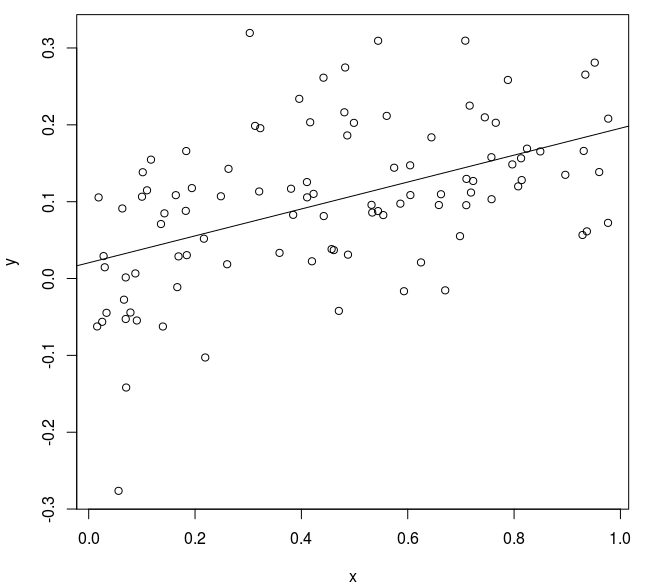
\includegraphics[width=0.55\columnwidth]{R_output.png}
\end{figure}
\end{onlyenv}
\end{overlayarea}
\end{frame}

\begin{frame}[t, fragile]{\subsecname}{基本操作}
\begin{itemize}
  \hilite<1> \item 第二种方式是将脚本代码写在文件中,然后一次性运行
  \hilite<2> \item 如果代码量很大建议使用第二种方式,因为文件比较容易修改和保存,而且目前
        有专用IDE可以辅助编写R脚本代码  
\end{itemize} 

\begin{overlayarea}{\textwidth}{\textheight}
\only<1>{
  \begin{figure}[ht]
    \centering
    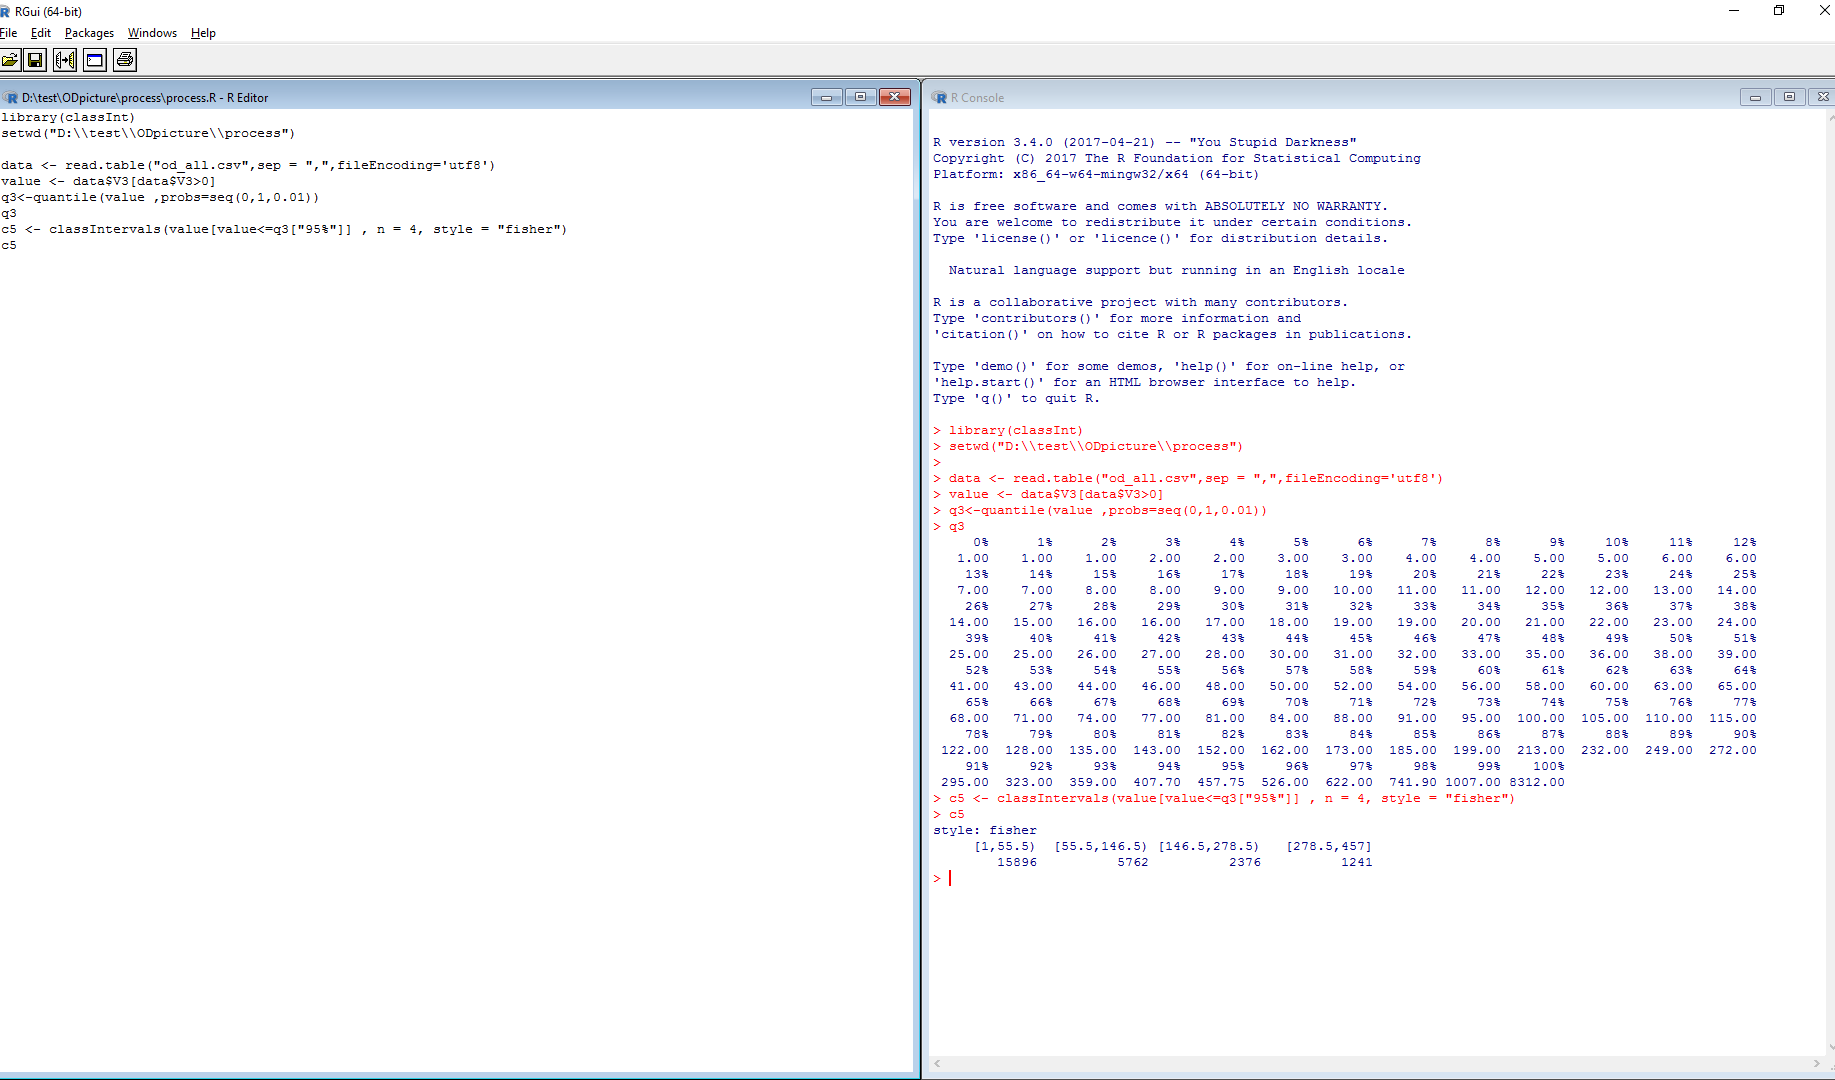
\includegraphics[width=0.8\columnwidth]{R_editor.png}
    \caption{在文本编辑器中编写脚本,然后一次性在终端运行}
  \end{figure}}   

\only<2>{
  \begin{figure}[ht]
    \centering
    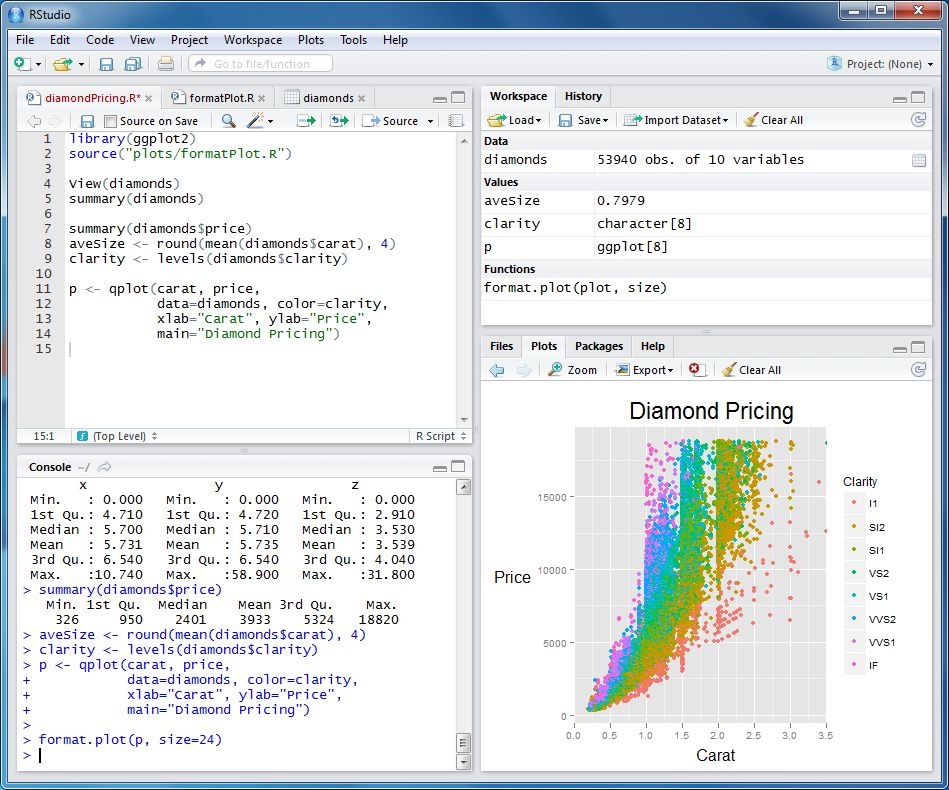
\includegraphics[width=0.6\columnwidth]{RStudio.jpg}
    \caption{\emphText{RStudio}是目前最专业的R IDE,具有大量针对R语言特点设计的功能,
             而且个人桌面版完全开源,可以免费使用}
  \end{figure}}   
\end{overlayarea}
\end{frame}

\begin{frame}[t]{\subsecname}{程序包}
  \begin{itemize}
    \hilite<1> \item R的程序包分为\emphText{base包}和\emphText{contrib包}
    \hilite<2> \item base包是安装R的时候就自带的,不需要单独安装,
    这类包的质量都非常高,性能稳定
    \hilite<3> \item contrib包是自愿者上传的,质量参次不齐;其中质量好
    且用户量大的扩展包有可能会纳入下一个版本的主程序包
  \end{itemize}

\begin{overlayarea}{\textwidth}{\textheight}
\only<1>{
  \begin{figure}[h]
    \centering
    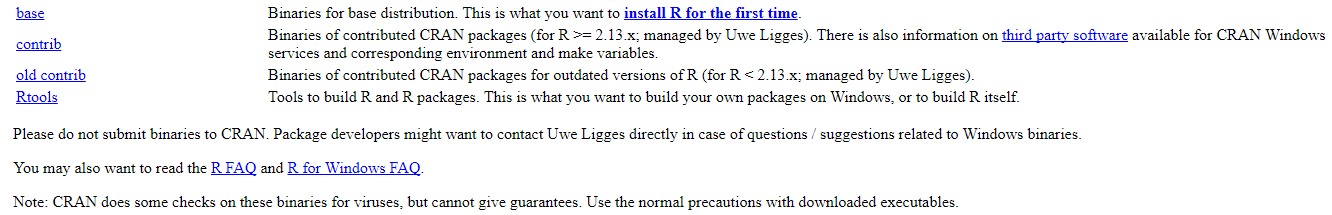
\includegraphics[width=\columnwidth]{R_packages.png}
    \caption{CRAN上下载base包和contrib包}
  \end{figure}}  

\only<2>{
  \begin{table} \centering \small
    \begin{tabular}{|c|c|}
      \toprule
      \rowcolor{LightCyan}
      名称 & 用途\\\hline
      base & R基础函数包\\\hline
      methods & 用于 R 对象和编程工具的方法和类的定义\\\hline
      datasets & R通用数据集\\\hline
      graphics & 基础统计绘图包 \\\hline
      utils & 通用函数包 \\\hline
      stats & 基础统计计算包 \\\hline
      grDevices & 基础或grid图形设备\\
      \bottomrule
    \end{tabular}
    \caption{常用的base包}
  \end{table}}

\only<3>{
  \begin{table} \centering \small 
    \begin{tabular}{|c|c|}
      \toprule
      \rowcolor{LightCyan}
      名称 & 用途\\\hline
      cluster & 聚类分析包\\\hline
      maptools & 空间数据读取和处理包\\\hline
      spatstat & 空间点数据分析包\\\hline
      sp & 空间数据基础类包\\\hline
      spdep & 空间自相关模型包\\\hline
      ggplot2 & 基于绘图语法的数据可视化包 \\\hline
      knitr & R文学编程包 \\\hline
      \bottomrule
    \end{tabular}
    \caption{常用的contrib包}
  \end{table}}
\end{overlayarea}
\end{frame}

\begin{frame}[t,fragile]{\subsecname}{程序包}
  \begin{itemize}
    \hilite<1> \item base包在R启动之后自动加载,可以直接使用;而contrib包则需要通过library函数调用,如果未安装
               相应包则会报错
    \hilite<2> \item 通过\emphTextStep{2-}{install.packages}函数安装contrib包
  \end{itemize}

\begin{overlayarea}{\textwidth}{\textheight}
\begin{onlyenv}<1->
\begin{rcode}
> library(sp)
Error in library(sp) : there is no package called ‘sp’
\end{rcode}
\end{onlyenv}

\begin{onlyenv}<2>
\begin{rcode}
> install.packages("sp")
Installing package into ‘/home/mono/Softwares/R/3.4’
(as ‘lib’ is unspecified)
--- Please select a CRAN mirror for use in this session ---
trying URL 'http://mirrors.tuna.tsinghua.edu.cn/CRAN/src/contrib/sp_1.2-6.tar.gz'
Content type 'application/octet-stream' length 1133739 bytes (1.1 MB)
==================================================
downloaded 1.1 MB

* installing *source* package ‘sp’ ...
\end{rcode}
\end{onlyenv}
\end{overlayarea}
\end{frame}

\begin{frame}[t,fragile]{\subsecname}{帮助系统}
  \begin{itemize}
    \hilite<1> \item 通过\emphTextStep{1-}{?命令}或者\emphTextStep{1-}{help函数}
               查看程序包中函数的本地帮助文档
    \hilite<2> \item 通过\emphTextStep{2-}{help.search函数}在整个帮助系统中进行关键字搜索
    \hilite<3> \item \emphTextStep{3-}{find函数}可以根据名称精确查找对象,
               \emphTextStep{3-}{apropos函数}可以根据名称模糊查找对象
  \end{itemize}

\begin{overlayarea}{\textwidth}{\textheight}
\begin{onlyenv}<1>
\begin{rcode}
> ?lm
lm               package:stats            R Documentation

Fitting Linear Models

Description:

     ‘lm’ is used to fit linear models.  It can be used to carry out regression, single stratum analysis of variance and analysis of covariance (although ‘aov’ may provide a more convenient interface for these).

Usage:

     lm(formula, data, subset, weights, na.action, method = "qr", model = TRUE, x = FALSE, y = FALSE, qr = TRUE, singular.ok = TRUE, contrasts = NULL, offset, ...)
\end{rcode}
\end{onlyenv}

\begin{onlyenv}<2>
\begin{rcode}
> help.search("data input")
Help files with alias or concept or title matching ‘data input’ using fuzzy matching:


utils::read.DIF         Data Input from Spreadsheet
utils::read.table       Data Input


Type '?PKG::FOO' to inspect entries 'PKG::FOO', or 'TYPE?PKG::FOO' for entries like 'PKG::FOO-TYPE'.
\end{rcode}
\end{onlyenv}

\begin{onlyenv}<3>
\begin{rcode}
> find("lm")
[1] "package:stats"
> appropos("lm")
 [1] "colMeans"        ".colMeans"       "confint.lm"      "contr.helmert"  
 [5] "dummy.coef.lm"   "getAllMethods"   "glm"             "glm.control"    
 [9] "glm.fit"         "KalmanForecast"  "KalmanLike"      "KalmanRun"      
[13] "KalmanSmooth"    "kappa.lm"        "lm"              ".lm.fit"        
[17] "lm.fit"          "lm.influence"    "lm.wfit"         "model.matrix.lm"
[21] "nlm"             "nlminb"          "predict.glm"     "predict.lm"     
[25] "residuals.glm"   "residuals.lm"    "summary.glm"     "summary.lm" 
\end{rcode}
\end{onlyenv}

\end{overlayarea}
\end{frame}

\subsection{数据操作}
\begin{frame}[t]{\subsecname}{对象(object)}
  \begin{itemize}
  \item R语言中操作的实体在技术上来说就是对象(object) 
  \item 语言中使用对象的好处是可以复用,提升自动化程度
  \item R的所有对象有两个内在属性:类型(mode)和长度(length)
  \end{itemize}

  \begin{columns}
    \begin{column}{.5\textwidth}
      \begin{figure}
        \centering 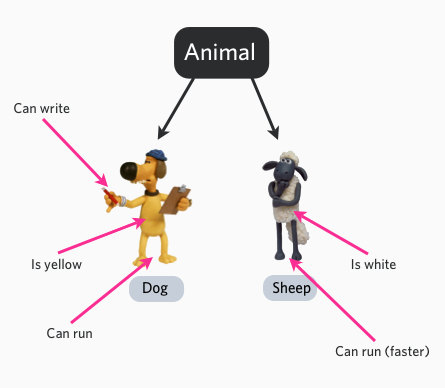
\includegraphics[width=\columnwidth]{object.png}
      \end{figure}
    \end{column}

    \begin{column}{.48\textwidth}
      \begin{ornamentblock}
        \centering
        {在R语言中,\emphText{几乎任何东西都是对象}}
      \end{ornamentblock}
    \end{column}
  \end{columns}
\end{frame}

\begin{frame}[t, fragile]{\subsecname}{数据类型(mode)}
  \begin{itemize}
  \item 实数型(real):整数(integer)、单精度(single)、双精度(double)
  \item 虚数型(complex):如10+21i
  \item 字符型(character, string):如"hello world"
  \item 逻辑型(logical):TRUE(可以简写成T),FALSE(可以简写成F)
  \item 函数(function)
  \item 表达式(expression)
  \end{itemize}

\begin{overlayarea}{\textwidth}{\textheight}
\begin{rcode}
> x <- 1
> mode(x)
[1] "numeric"
> length(x)
[1] 1
> A <- "Gomphotherium"; compar <- TRUE; z <- 1i
> mode(A); mode(compar); mode(z)
[1] "character"
[1] "logical"
[1] "complex"
# 表达式
> x <- 3; y <- 2.5; z <- 1
> exp1 <- expression(x / (y + exp(z)))
> exp1
expression(x/(y + exp(z)))
> eval(exp1)
[1] 0.5749019
\end{rcode}
\end{overlayarea}
\end{frame}

\begin{frame}[t]{\subsecname}{数据结构}
  \begin{itemize}
  \item R语言中为了提高数据的使用效率,预定义了专门用于表示数据的对象,也就是数据结构,这些数据结构支撑了R强大的统计分析能力
  \end{itemize}
% \only<1>{
%   \begin{ornamentblock}[userdefinedwidth=0.6\textwidth,align=center]
%         \centering
%         {Everything in R is an object\\
%          Every object in R has a class}
%       \end{ornamentblock}}
  \begin{table} \centering \small
    \begin{tabular}{|c|c|}
      \toprule
      \rowcolor{LightCyan}
      数据结构 & 类型\\\hline
      向量(vector) & 数值型,字符型,复数型,逻辑型\\\hline
      因子(factor) & 数值型,字符型\\\hline
      数组(array) & 数值型,字符型,复数型,逻辑型\\\hline
      矩阵(matrix) & 数值型,字符型,复数型,逻辑型 \\\hline
      数据框(data.frame) & 数值型,字符型,复数型,逻辑型 \\\hline
      列表(list) & 任意其他类型 \\\hline
      时间序列(ts) & 数值型,字符型,复数型,逻辑型\\
      \bottomrule
    \end{tabular}
    \caption{R基础数据结构}
  \end{table}
\end{frame}

\begin{frame}[t,fragile]{\subsecname}{数据结构}
  \frametitle{}{向量(vector)}
  \begin{itemize}
  \item \emphText{向量是R中最基本的数据单元},向量中的对象类型必须相同
  \item 构建向量常用的函数: rep()、c()、seq()、cbind()、rbind()等
  \item \emphText{向量的下标从1开始},这和其他计算机高级编程语言是不一样的!
  \end{itemize}  

%\begin{overlayarea}{\textwidth}{\textheight}
\begin{rcode}
> x <-1:10; x
[1]  1  2  3  4  5  6  7  8  9 10
> x[3]
[1] 3
> c(7.11, 9.11, 9.19, 1.23)
[1] 7.11 9.11 9.19 1.23
> c("B", "A")
[1] "B" "A"
> rep(1, 10)
[1] 1 1 1 1 1 1 1 1 1 1
> seq(1, 5, 0.5)
[1] 1.0 1.5 2.0 2.5 3.0 3.5 4.0 4.5 5.0
> cbind(0, rbind(1, 1:3))
     [,1] [,2] [,3] [,4]
[1,]    0    1    1    1
[2,]    0    1    2    3
\end{rcode}  
%\end{overlayarea}
\end{frame}

\begin{frame}[t,fragile]{\subsecname}{数据结构}
  \frametitle{}{因子(factor)}
  \begin{itemize}
  \item 因子是对应统计学中的分类数据(categorical data)而设计的
  \item 因子形式上是一个对等长的向量元素进行分类(分组)的向量对象
  \item 因子数据具有水平(level)和标签(label),前者即分类变量的不同取
值,后者即各类取值的名称
  \end{itemize}  

\begin{rcode}
> factor(1:3, labels=c("A", "B", "C"))
[1] A B C
Levels: A B C
> (x = factor(c(1, 2, 3, 1, 1, 3, 2, 3, 3), levels = 1:3,
+   labels = c("g1", "g2", "g3")))
[1] g1 g2 g3 g1 g1 g3 g2 g3 g3
Levels: g1 g2 g3
\end{rcode}  
\end{frame}

\begin{frame}[t,fragile]{\subsecname}{数据结构}
  \frametitle{}{数组(array)和矩阵(matrix)}
  \begin{itemize}
  \item 数组和矩阵是具有维度属性(dimension)的数据结构,
        实质是有附加属性(维数dim)的向量
  \item 矩阵是数组的特例,它的维度为2,用来指定行数和列数
  \end{itemize}  

\begin{rcode}
# 二维矩阵
> matrix(data=5, nr=2, nc=2)
     [,1] [,2]
[1,]    5    5
[2,]    5    5
# 三维数组
> array(1:24, c(3, 4, 2))
, , 1
     [,1] [,2] [,3] [,4]
[1,]    1    4    7   10
[2,]    2    5    8   11
[3,]    3    6    9   12

, , 2
     [,1] [,2] [,3] [,4]
[1,]   13   16   19   22
[2,]   14   17   20   23
[3,]   15   18   21   24
\end{rcode}  
\end{frame}

\begin{frame}[t,fragile]{\subsecname}{数据结构}
  \frametitle{}{列表(list)}
  \begin{itemize}
  \item 列表是一种灵活的数据结构,\emphText{用于生成包含不同类型对象的集合}
  \end{itemize}  

\begin{rcode}
# 创建list
> x <- 1:4; y <- 2:4; L1 <- list(A=x, B=y); L1
$A
[1] 1 2 3 4

$B
[1] 2 3 4
# list元素的引用
> L1[[1]]
[1] 1 2 3 4
> L1["A"]
$A
[1] 1 2 3 4
> L1[["A"]]
[1] 1 2 3 4
> L1$B
[1] 2 3 4
\end{rcode}  
\end{frame}

\begin{frame}[t,fragile]{\subsecname}{数据结构}
  \frametitle{}{数据框(data.frame)}
  \begin{itemize}
  \item 数据框是由许多向量组成的一个二维的对象,主要用于保存建模所需要的数据
  \item 数据框的实质是一个“整齐的”列表,它只要求各列内的数据类型相同,而列之间的可以不同
  \item \emphText{数据框是R中最重要的一种数据结构},大多数数据都是以数据框形式输到R中的
  \end{itemize}  

\begin{rcode}
# 创建数据框
# 数据框中的向量必须有相同的长度,如果其中有一个比其它的短,它将“循环”整数次(以使得其长度与其它向量相同)
> x <- 1:4; M <- c(10, 35); y <- 2:4
> data.frame(x, M)
  x  M
1 1 10
2 2 35
3 3 10
4 4 35
> data.frame(x, y)
Error in data.frame(x, y) :
   arguments imply differing number of rows: 4, 3
\end{rcode}  
\end{frame}

\begin{frame}[t,fragile]{\subsecname}{数据输入输出}
  \begin{itemize}
    \hilite<1> \item R的数据可以按照数据结构手动输入,也可以通过读取外部文件自动输入
    \hilite<2> \item R base包提供了文本文件(ASCII)的读取函数:\emphTextStep{2-}{read.table}、
                     \emphTextStep{2-}{scan}和\emphTextStep{2-}{read.fwf}等
    \hilite<3> \item R base包也提供了文本文件(ASCII)的输出函数:\emphTextStep{2-}{write.table}
    \hilite<4> \item 另外,\emphTextStep{4-}{图形作为对象也可以输出},这将在后面会专门介绍
  \end{itemize}

\begin{overlayarea}{\textwidth}{\textheight}
\begin{onlyenv}<2>
%\begin{minted}{R}
\begin{rcode}
# 从外部读取data.dat文件,并且将数据赋给一个名为mydata的对象,这里mydata是一个data.frame数据结构
> mydata <- read.table("data.dat")

# read.table的参数
read.table(file, header = FALSE, sep = "", quote = "\"’", dec = ".", row.names, col.names, as.is = FALSE, na.strings = "NA",colClasses = NA, nrows = -1,skip = 0, check.names = TRUE, fill =!blank.lines.skip,strip.white = FALSE, blank.lines.skip = TRUE,comment.char = "#")
\end{rcode}
%\end{rcode}
\end{onlyenv}

\begin{onlyenv}<3>
\begin{rcode}
# 函数write.table可以在文件中写入一个对象,一般是写一个数据框,也可以是其它类型的对象
write.table(x, file = "", append = FALSE, quote = TRUE, sep = " ", eol = "\n", na = "NA", dec = ".", row.names = TRUE, col.names = TRUE, qmethod = c("escape", "double"))
\end{rcode}
\end{onlyenv}

\end{overlayarea}
\end{frame}

\subsection{程序控制}
\begin{frame}{\subsecname}{控制语句}
  \begin{itemize}
  \item<1-> if (条件) {表达式}
  \item<1-> if (条件) {表达式} else {表达式}
  \item<1-> if...else if...else if... else...
  \item<1-> ifelse (条件, yes, no)
  \item<2-> for (变量 in 向量) {表达式}
  \item<2-> while (条件) {表达式} 
  \end{itemize}

\onslide<3>{
\begin{badbox}{}
循环的编程模式在R中效率很低,尽量避免使用!
\end{badbox}} 
\end{frame}

\subsection{函数}
\begin{frame}[t,fragile]{\subsecname}{}
  \begin{itemize}
  \item R语言中可以定义函数,以便编程中可以以不同的参数值重复使用同一段代码
  \item 定义函数的方式为:function(arglist) expr return(value);
其中arglist是参数列表,expr是函数的主体,return()用来返回函数值
\item \emphText{函数是R中用于黑箱操作的重要实体}
  \end{itemize}  

\begin{rcode}
# 定义峰度函数kurtosis,该函数有两个参数,数据向量x和是否删除缺失值na.rm,后者有默认值FALSE
> kurtosis = function(x, na.rm = FALSE) {
+   if (na.rm)
+     x = x[!is.na(x)]
+   return(sum((x - mean(x))^4)/(length(x) * var(x)^2) - 3)
+ }
> # 引用函数
> kurtosis(runif(100))
[1] -1.36086
\end{rcode}  
\end{frame}

\subsection{公式和表达式}
\begin{frame}[t, fragile]{\subsecname}{}

\end{frame}

\subsection{面向对象编程}
\begin{frame}[t]{\subsecname}{}
\begin{itemize}
\item \emphText{R语言中支持面向对象(Object-Oriented, OO)编程来提高代码的使用率},从而实现具体功能的扩展和模块化
  \item R语言作为一种统计编程语言,需要用的OO的场景主要有以下两类:
  \begin{itemize}
     \item[\PencilLeftDown] 当需要用一种新的类型来表示数据,该类型与
   已有的数据类型有区别的时候
     \item[\PencilLeftDown] 当需要一个新的函数,该函数可以根据不同的
参数类型做出不同的反应的时候
  \end{itemize}
\item R语言中有四种OO的实现系统:\emphText{S3、S4、RC(R5)和R6}
\end{itemize}  
\end{frame} 

\begin{frame}[t,fragile]{\subsecname}{S3系统}
  \begin{itemize}
  \item S3是R语言的第一种也是最简单的一种OO系统,也是\emphText{CRAN程序包中最常用的一种OO系统}
  \item S3系统中方法(method)是属于函数而不是属于类,这种函数称为\emphText{泛型函数}(generic function)
  \item 泛型函数的形式是\emphText{generic.class()},其实质是根据传入函数的第一个参数的类去调用相应的“子函数”
  \end{itemize}  

  %\begin{overlayarea}{\textwidth}{\textheight}
\begin{rcode}
> library(pryr) # 调用pryr程序包检测某个方法是否是S3系统
> df <- data.frame(x = 1:10, y = letters[1:10])
> otype(df)    # data.frame是一个S3方法
[1] "S3"
# 调用methods()来查看属于某个泛型的所有方法
> methods("mean")
[1] mean.Date   mean.default    mean.difftime   mean.POSIXct    mean.POSIXlt
# 根据传入函数的第一个参数的类去调用相应的“子函数”
> (today <- Sys.Date())
[1] "2018-01-18"
> tenweeks <- seq(today, length.out=10, by="1 week")
> class(tenweeks)
[1] "Date"
> mean(tenweeks) # 这里调用的实际上是mean.Date
[1] "2018-02-18" 
\end{rcode}  
  %\end{overlayarea}
\end{frame}

\begin{frame}[t,fragile]{\subsecname}{S3系统}
  \begin{itemize}
  \item<1-> 创建S3对象最简单的方法是给一个变量增加\emphText{class属性};也可以通过\emphText{structure()}函数创建
  \item<2-> 使用\emphText{UseMethod()}函数定义S3型泛型函数
  \item<3-> 通过\emphText{NextMethod()}函数实现继承
  \end{itemize}  

\begin{overlayarea}{\textwidth}{0.5\textheight}
\begin{onlyenv}<1>
\begin{rcode}
# 通过给变量增加class属性来创建S3型对象
> x <- 1; attr(x,'class') <- 'foo'
> x
[1] 1
attr(,"class")
[1] "foo"
> otype(x)
[1] "S3"
# 通过structure函数来创建S3型对象
> y <- structure(2, class='foo')
> y
[1] 2
attr(,"class")
[1] "foo"
> otype(y)
[1] "S3"
\end{rcode}  
\end{onlyenv}

\begin{onlyenv}<2>
\begin{rcode}
# 用UseMethod定义S3泛型函数
> teacher <- function(x,...) UseMethod("teacher")
# 定义了三个teacher的内部函数
> teacher.lecture <- function(x) print("上课")
> teacher.assignment <- function(x) print("布置作业")
> teacher.default <- function(x) print("你不是老师")
# 定义一个S3对象a,其class是lecture
> a <- structure('A', class='lecture')
# teacher泛型函数根据传入的类调取teacher.lecture()函数
> teacher(a) 
[1] "上课"
# 默认泛型函数
> teacher()
[1] "你不是老师"
\end{rcode}  
\end{onlyenv}

\begin{onlyenv}<3>
\begin{rcode}
# 定义一个S3泛型函数node
> node <- function(x) UseMethod('node', x)
# 定义node的内部函数,其中son函数通过NextMethod()指向father
> node.default <- function(x) "Default node"
> node.father <- function(x) c("father")
> node.son <- function(x) c("son", NextMethod())
# 定义对象n有两个class,调用node函数会先执行son函数,再执行father函数,模拟了子函数调用父函数的过程
> n <- structure(1, class = c("son", "father"))
> node(n)
[1] "son"    "father"
\end{rcode}
\end{onlyenv}

\begin{onlyenv}<4>
\begin{badbox}{S3系统的缺点}
\begin{itemize}
\item[\PencilLeftDown] S3系统并不是真正的OO,只是通过函数来模拟OO
\item[\PencilLeftDown] S3系统使用简单,但是很难处理复杂的对象关系
\item[\PencilLeftDown] S3系统的内部函数并没有真正封装,可以绕过泛型函数检查直接被调用
\item[\PencilLeftDown] S3系统的class属性可以被任意设置,没有检查机制
\end{itemize}
\end{badbox}
\end{onlyenv}
\end{overlayarea}
\end{frame}

\begin{frame}[c,fragile]{\subsecname}{S4系统}
  \begin{itemize}
  \item<1-> 相比S3系统,S4系统有更明确和严谨的OO系统特征
  \item<2-> S4有专门的类定义函数\emphText{setClass()}和类的实例化函数\emphText{new()}
  \item<3-> 对象类型检查函数\emphText{setValidity()}
  \item<4-> S4泛型函数实现了方法定义和实现的分离,通过\emphText{setGeneric()}函数定义接口,
    \emphText{setMethod()}函数定义实现方法;\emphText{standardGeneric}定义泛型函数,
类似S3中的UseMethod
  \end{itemize}  

\begin{overlayarea}{\textwidth}{\textheight}
\begin{onlyenv}<2>
\begin{rcode}
# 定义S4类person以及person的子类son
> setClass('person',slots=list(name="character",age="numeric"))
> setClass("son", slots=list(father="person",mother="person"),contains="person")
# 实例化对象
> father <- new("person",name="F",age=44)
> mother <- new("person",name="M",age=42)
> son <- new("son",name="S",age=16,father=father,mother=mother)
# 查看son对象的属性
> son@father
An object of class "person"
Slot "name":
[1] "F"

Slot "age":
[1] 44
\end{rcode}  
\end{onlyenv}

\begin{onlyenv}<3>
\begin{rcode}
# 定义S4类person
> setClass('person',slots=list(name="character",age="numeric"))
# 传入错误的age类型
> bad <- new("person",name="bad",age="aaa")
Error in validObject(.Object) : 
  invalid class “person” object: invalid object for slot "age" in class "person": got class "character", should be or extend class "numeric"
# 设置age属性的非负检查
> setValidity("person",function(object){
+    if(object@age <=0) stop("Age is negative.")
+ })
# 传入age属性小于0时会报错
> bad2 <- new("person",name="bad",age=-1)
Error in validityMethod(object) : Age is negative.
\end{rcode}
\end{onlyenv}

\begin{onlyenv}<4>
\begin{rcode}
# 定义person类,slots参数定义类的属性
> setClass('person',slots=list(name="character",age="numeric"))
# 定义泛型函数work,即接口
> setGeneric("work",function(obj) standardGeneric("work"))
[1] "work"
# 定义work的实现函数,并指定参数类型为person
> setMethod("work",signature(obj="person"),function(obj) cat(obj@name, "is working"))
[1] "work"
# 创建person类型对象a,并将其传入work函数
> a <- new("person",name="Conan",age=16)
> work(a)
Conan is working
\end{rcode}  
\end{onlyenv}
\end{overlayarea}
\end{frame}

\begin{frame}[t,fragile]{\subsecname}{RC和R6系统}
  \begin{itemize}
  \item<1-> RC(Reference classes),又称为R5,是从2.12版本引入的新一代OO系统
  \item<2-> \emphText{RC系统的方法是在类中定义的},而不是通过泛型函数
  \item<2-> RC系统依赖于S4系统,是对OO的进一步封装,已经非常趋于主流编程语言中的OO实现
  \item<3-> R6是一个\emphTextStep{3}{完全独立的R程序包},类似RC但不依赖于S4系统 
  \end{itemize}  

\begin{overlayarea}{\textwidth}{\textheight}
\begin{onlyenv}<2>
\begin{rcode}
# 定义一个RC类,方法包括在定义中
> user<-setRefClass("user",
+      fields=list(name="character",favorite="vector"), 
+      methods=list(                                                      
+             addFavorite=function(x){
+                 favorite<<-c(favorite,x)},
+             delFavorite=function(x){
+                 favorite<<-favorite[-which(favorite==x)]}))
# 实例化一个u对象
> u <- user$new(name="u",favorite=c('movie','football'))
# 操作方法
> u$addFavorite('shopping')
> u$favorite
[1] "movie"    "football" "shopping"
\end{rcode}  
\end{onlyenv}
\end{overlayarea}
\end{frame}
%%%%%%%%%%%%%%%%%%%%%%%%%%%%%%%%%%%%%%%%%%%%%%%%%%%%%%%%%
\section{R绘图}
%%%%%%%%%%%%%%%%%%%%%%%%%%%%%%%%%%%%%%%%%%%%%%%%%%%%%%%%%%%%
\subsection{绘图基础知识}
\begin{frame}[t, fragile]{\subsecname}{绘图设备}
  \begin{itemize}
  \item<1-> 绘图设备用于管理R的图形输出,分为\emphText{窗口设备和图形设备}
  \item<2-> 窗口设备通过一个依赖于\emphTextStep{2-}{操作系统底层窗口来输出图形},在Unix/Linux系统中称为X11,在
        Windows系统中称为windows
  \item<2-> 图形设备用于将\emphTextStep{2-}{R对象输出到文件},例如jpeg、pdf、png、bmp、metafile等
  \item<3-> \emphTextStep{3-}{layout()}函数用于将绘图设备进行分割,
            图形将一次显示在不同的部分中;不再使用的绘图设备用\emphTextStep{3-}{dev.off()}函数关闭 
  \end{itemize} 

\begin{overlayarea}{\textwidth}{\textheight}
\begin{onlyenv}<2>
\begin{rcode}
# 开启三个绘图设备,X11函数用于开启窗口设备,pdf和jpeg函数用于输出图形到文件
> |\colorbox{green}{x11();pdf();jpeg()}|
> dev.list()
X11cairo      pdf     jpeg 
       2        3        4 
# 关闭2号绘图设备
> dev.off(2) 
\end{rcode}  
\end{onlyenv}

\begin{onlyenv}<3>
      \begin{columns}
        \begin{column}{.4\textwidth}
          \begin{figure}
            \centering
            
\includegraphics[width=0.8\columnwidth]{layout.png}
          \end{figure}
        \end{column}

        \begin{column}{.6\textwidth}
 \centering
\begin{rcode}
> mat <- matrix(1:4, 2, 2)
> layout(mat)
> layout.show(4)
\end{rcode}
        \end{column}
      \end{columns}
\end{onlyenv}

\begin{onlyenv}<4>
      \begin{columns}
        \begin{column}{.4\textwidth}
          \begin{figure}
            \centering
            \includegraphics[width=0.8\columnwidth]{layout2.png}
          \end{figure}
        \end{column}

        \begin{column}{.6\textwidth}
 \centering
\begin{rcode}
> mat <- matrix(c(1:3, 3), 2, 2)
> layout(mat)
> layout.show(3)
\end{rcode}
        \end{column}
      \end{columns}
\end{onlyenv}
\end{overlayarea}
\end{frame} 

\begin{frame}[t,fragile]{\subsecname}{绘图函数}
\begin{itemize}
\item R中的统计图形都是由相应的绘图函数生成,其包含了统计图形中各种细节的设置
\item 绘图函数分为\emphText{高级绘图函数和低级绘图函数}
\item 高级绘图函数用于快速绘制常见的统计图形,
低级绘图函数用于在高级绘图函数绘制的统计图形基础上进行个性化的定制
\end{itemize}

\begin{overlayarea}{\textwidth}{\textheight}
\begin{onlyenv}<2>
\begin{columns}
        \begin{column}{.4\textwidth}
          \begin{figure}
            \centering
            \includegraphics[width=\columnwidth]{高级绘图函数.png}
          \end{figure}
        \end{column}

        \begin{column}{.6\textwidth}
 \centering
\begin{rcode}
> x = runif(100); y = 0.2*x + 0.1*rnorm(100)
# 高级绘图函数plot绘制散点图
> plot(x, y)
\end{rcode}
        \end{column}
      \end{columns}
\end{onlyenv}

\begin{onlyenv}<3>
\begin{columns}
        \begin{column}{.4\textwidth}
          \begin{figure}
            \centering
            \includegraphics[width=\columnwidth]{低级绘图函数.png}
          \end{figure}
        \end{column}

        \begin{column}{.6\textwidth}
 \centering
\begin{rcode}
> x = runif(100); y = 0.2*x + 0.1*rnorm(100)
# 高级绘图函数plot绘制散点图
> plot(x, y)
# 回归模型拟合散点数据
> fit = lm(y ~ x)
# 低级绘图函数abline在原散点图基础上增加拟合直线
> |\colorbox{green}{abline(fit)}|
\end{rcode}
        \end{column}
      \end{columns}
\end{onlyenv}
\end{overlayarea}  
\end{frame}

\begin{frame}[t,fragile]{\subsecname}{绘图参数}
\begin{itemize}
\item<1-> 除了低级绘图函数之外,图形的显示也可以用绘图参数来定制
\item<2-> 绘图函数里面可以\emphTextStep{2-}{临时设置参数},不会影响后面其他绘图函数的效果
\item<3-> \emphTextStep{3-}{par()函数可以设置全局参数},全局参数只要绘图设备不关闭就会一直起作用
\end{itemize}

\begin{overlayarea}{\textwidth}{\textheight}
\begin{onlyenv}<2>
\begin{columns}
        \begin{column}{.4\textwidth}
          \begin{figure}
            \centering
            \includegraphics[width=\columnwidth]{plot.png}
          \end{figure}
        \end{column}

        \begin{column}{.6\textwidth}
 \centering
\begin{rcode}
> x<-rnorm(10); y<-rnorm(10)
# 通过设置plot函数的参数实现临时效果
> plot(x, y, xlab="Ten random values", ylab="Ten other values",xlim=c(-2, 2), ylim=c(-2, 2), pch=22, col="red", bg="yellow", bty="l", tcl=-.25, las=1, cex=1.5, main="通过plot函数的参数来定制散点图")
\end{rcode}
        \end{column}
      \end{columns}
\end{onlyenv}

\begin{onlyenv}<3>
\begin{columns}
        \begin{column}{.4\textwidth}
          \begin{figure}
            \centering
            \includegraphics[width=\columnwidth]{par.png}
          \end{figure}
        \end{column}

        \begin{column}{.6\textwidth}
 \centering
\begin{rcode}
# 缺省绘图参数被复制到opar对象
> opar <- par()
# 通过par()函数定制图形
> par(|\colorbox{green}{bg}|="lightyellow", |\colorbox{green}{col.axis}|="blue", |\colorbox{green}{mar}|=c(4, 4, 2.5, 0.25))
> plot(x, y, xlab="Ten random values", ylab="Ten other values",
+ xlim=c(-2, 2), ylim=c(-2, 2), pch=22, col="red", bg="yellow",
+ bty="l", tcl=-.25, las=1, cex=1.5)
# 通过低级绘图函数title为上图添加定制标题
> title("通过par参数来定制散点图", font.main=3, adj=1)
# 恢复缺省绘图参数
> par(opar)
\end{rcode}
        \end{column}
      \end{columns}
\end{onlyenv}
\end{overlayarea}  
\end{frame}

\begin{frame}{\subsecname}{绘图参数}
\only<1>{
  \begin{table} \centering \scriptsize
    \begin{tabular}{|c|c|}
      \toprule
      \rowcolor{LightCyan}
      参数名称 & 作用\\\hline
      adj & 调整图中文字的相对位置\\\hline
      bg,fg & 背景颜色和前景颜色\\\hline
      bty & 设置图形边框样式\\\hline
      cex & 图上元素(文本、符号等)的缩放倍数 \\\hline
      col & 图中符号的颜色 \\\hline
      family,font & 设置文本的字体族和字体样式 \\\hline
      lab,mgp & 设置坐标轴刻度数目和边界宽度\\\hline
      lend,ljoin & 线条末端样式和线条相交处的样式\\\hline
      lheight & 图中文本行高\\\hline
      lty,lwd & 线条样式和宽度\\\hline
      mar,oma,pty & 图形区域设置\\\hline
      pch & 点符号样式\\\hline
      srt & 字符串旋转角度\\\hline
      tck,tcl & 坐标轴刻度线高度\\
      \bottomrule
    \end{tabular}
    \caption{par函数的部分参数}
  \end{table}}  

\only<2>{
\begin{figure}[ht]
  \centering
  \includegraphics[width=0.8\columnwidth]{par-example.png}
  \caption{par函数参数效果示例}
\end{figure}}
\end{frame}

\begin{frame}{\subsecname}{绘图参数}
\only<1>{
  \begin{table} \centering \small
    \begin{tabular}{|c|c|}
      \toprule
      \rowcolor{LightCyan}
      参数名称 & 作用\\\hline
      type & 图形样式类型\\\hline
      main,sub & 主标题和副标题\\\hline
      xlab,ylab & 坐标轴标题\\\hline
      asp & 图形横轴比 \\\hline
      x,y & 散点图的两个向量 \\\hline
      xlim,ylim & 坐标系界限\\\hline
      axes & 是否画坐标轴\\\hline
      frame.plot & 是否给图形加框\\\hline
      panel.first & 作图前完成的工作\\\hline
      panel.last & 作图后要完成的工作\\
      \bottomrule
    \end{tabular}
    \caption{plot函数的部分参数}
  \end{table}}  

\only<2>{
\begin{figure}[ht]
  \centering
  \includegraphics[width=0.8\columnwidth]{plot-example.png}
  \caption{plot函数参数type的九种效果示例}
\end{figure}}
\end{frame}

\subsection{绘图元素拆解}
\begin{frame}{\subsecname}{}
  \begin{columns}
    \begin{column}{.4\textwidth}
      \begin{figure}
        \centering \includegraphics[width=\columnwidth]{庖丁解牛.jpg}
      \end{figure}
    \end{column}

    \begin{column}{.6\textwidth}
      \begin{ornamentblock}
        { 庖丁为文惠君解牛,手之所触,肩之所倚,足之所履,膝之所踦,砉然向然,奏刀騞然,莫不中音。\\
          \rightline{\textemdash《庄子·养生主》}}
      \end{ornamentblock}
    \end{column}
  \end{columns}
\end{frame}

\begin{frame}[t]{\subsecname}
\begin{itemize}
\item<1-> 统计图形的所有元素都可以在R语言中\emphText{通过低级绘图函数进行定制}
\end{itemize}

\begin{overlayarea}{\textwidth}{\textheight}
  \begin{table} \centering \small
    \begin{tabular}{|c|c|}
      \toprule
      \rowcolor{LightCyan}
      统计图形元素 & 常用函数\\\hline
      图形区域 & par\\\hline
      颜色 & colors,palette,rgb,rainbow\\\hline
      点 & points\\\hline
      线 & lines,abline,arrows,segments,xspline\\\hline
      面 & polygon,rect,box \\\hline
      网格线 & grid \\\hline
      文本 & text,title,mtext \\\hline
      图例 & legend\\\hline
      坐标轴 & axis \\   
      \bottomrule
    \end{tabular}
    \caption{统计图形的要素}
  \end{table}
\end{overlayarea}  
\end{frame}

\begin{frame}[t]{\subsecname}{图形区域}
\begin{itemize}
\item R的绘图设备分为三个区域:\emphText{作图区域(Plot Region)、图形区域(Figure Region)和设备区域(Device Region)}
\item 这三个区域对应两个边界:\emphText{图形边界(Figure Margin)和外边界(Outer Margin)};图形边界由par函数的\emphText{mar参数}设置,外边界由\emphText{oma参数}设置
\end{itemize}  

\begin{figure}
  \centering
  \includegraphics[width=0.5\columnwidth]{plot_region.png}
  \caption{最大的灰色区域是\emphText{设备区域},设备区域内的白色实框区域是\emphText{图形区域},
最里面的灰色虚框区域是\emphText{作图区域},\emphText{所有的统计图形都是在作图区域内绘制}}
\end{figure}
\end{frame}

\begin{frame}[t]{\subsecname}{颜色}
\begin{itemize}
\item<1-> R中颜色的设置由grDevices包支持,提供了大量颜色函数
\item<2-> 颜色函数分\emphTextStep{2}{为固定颜色选择函数、颜色生成函数和转换函数和特定颜色主题调色板}
\end{itemize}

\begin{figure}
  \centering
  \includegraphics[width=0.7\columnwidth]{colors-example.png}
  \caption{R中的颜色} 
\end{figure}  
\end{frame}

\begin{frame}[t,fragile]{\subsecname}{颜色}
\begin{itemize}
\item<1-> 固定颜色选择函数:\emphText{colors()}、\emphText{palette()}
\item<2-> colors()函数直接通过英文名称来调取预设颜色
\item<3-> palette()函数用来设置调色板或者获得调色板颜色值。和colors不同的是palette函数结果并不是固定颜色;
但是只要一旦设置了调试板,它的取值在下一次设置前会一直保存
\end{itemize}

\begin{overlayarea}{\textwidth}{\textheight}
\begin{onlyenv}<2>
  \begin{columns}
    \begin{column}{.4\textwidth}
\centering
      \begin{figure}
        \includegraphics[width=\columnwidth]{colors-bar.png} 
      \end{figure}
    \end{column}

    \begin{column}{.6\textwidth}
\centering
\begin{rcode}
# 通过colors函数随机生成20种预设颜色
> sample(colors(), 20)
 [1] "tomato"       "lightcyan4"   "navajowhite1" "gray5"        "seagreen3"   
 [6] "ghostwhite"   "grey60"       "cornsilk4"    "linen"        "darkblue"    
[11] "gray26"       "steelblue1"   "grey"         "plum4"        "violet"      
[16] "gray83"       "red"          "thistle1"     "palegreen4"   "oldlace" 
\end{rcode}
    \end{column}
  \end{columns}
\end{onlyenv}

\begin{onlyenv}<3>
\begin{rcode}
# palette默认颜色
> palette()
[1] "black"   "red"     "green3"  "blue"    "cyan"    "magenta" "yellow" 
[8] "gray" 

# 更改后的调色板颜色
> palette(colors()[1:10])
> palette()
 [1] "white"         "aliceblue"     "antiquewhite"  "antiquewhite1"
 [5] "antiquewhite2" "antiquewhite3" "antiquewhite4" "aquamarine"   
 [9] "aquamarine"    "aquamarine2"  

> # 恢复默认调色板
> palette("default")
> palette()
[1] "black"   "red"     "green3"  "blue"    "cyan"    "magenta" "yellow" 
[8] "gray" 
\end{rcode}
\end{onlyenv}
\end{overlayarea}  
\end{frame}

\begin{frame}[t,fragile]{\subsecname}{颜色}
\begin{itemize}
\item R中还提供利用颜色生成原理构造颜色,如RGB模型(红绿蓝三原色)、
          HSV色彩模型(色调、饱和度和纯度)、HCL色彩模型(色调、色度和亮度)等
\item 对应的颜色生成和转换函数:\emphText{rgb()}、\emphText{hsv()}、
      \emphText{hcl()}、\emphText{gray()}等
\end{itemize}

\begin{overlayarea}{\textwidth}{\textheight}
\begin{onlyenv}<2>
\begin{rcode}
# 在rgb()函数中用一元线性函数控制绿色在[0, 1]上的取值,同时将红色和蓝色分别控制为1和0,那么我们将得到从纯红色到黄色的一个颜色渐变
> (x = rgb(1, seq(0, 1, length = 20), 0))
 [1] "#FF0000" "#FF0D00" "#FF1B00" "#FF2800" "#FF3600" "#FF4300" 
 [7] "#FF5100" "#FF5E00" "#FF6B00" "#FF7900" "#FF8600" "#FF9400" 
[13] "#FFA100" "#FFAE00" "#FFBC00" "#FFC900" "#FFD700" "#FFE400" 
[19] "#FFF200" "#FFFF00"
> barplot(rep(1, 20), col = x)
\end{rcode}
\begin{figure}\centering
  \includegraphics[width=0.8\columnwidth]{rgb-bar.png}
\end{figure}
\end{onlyenv}

\begin{onlyenv}<3>
\begin{rcode}
# 利用rgb()函数的透明度参数alpha生成半透明的显示效果
> library(MSG)
> data(BinormCircle)
> par(mfrow = c(1, 2), pch = 20, ann = FALSE, mar = c(2, 2 + 2, 0.5, 0.2))
> plot(BinormCircle, col = rgb(1, 0, 0))
> plot(BinormCircle, col = rgb(1, 0, 0, |\colorbox{green}{alpha}| = 0.01))
\end{rcode}
\begin{figure}\centering
  \includegraphics[width=0.9\columnwidth]{color-example.png}
\end{figure}
\end{onlyenv}
\end{overlayarea}  
\end{frame}

\begin{frame}[t,fragile]{\subsecname}{颜色}
\begin{itemize}
\item 由于基于颜色生成原理构造颜色过于专业,因此R中还提供了一种比较简单的\emphText{特定颜色主题调试板}
\item 特定颜色主题调试板用\emphText{渐变的颜色}来表现特定的主题
\end{itemize}

\begin{overlayarea}{\textwidth}{\textheight}
\only<1>{
  \begin{table} \centering \small
    \begin{tabular}{|m{0.2\columnwidth}|m{0.7\columnwidth}|}
      \toprule
      \rowcolor{LightCyan}
      函数名称 & 效果\\\hline
      rainbow() & 彩虹颜色(红橙黄绿青蓝紫)\\\hline
      heat.colors() & 从红色渐变到黄色再变到白色,适合表示“高温”、“白热化”\\\hline
      terrain.colors() & 从绿色渐变到黄色再到棕色最后到白色,适合表示地理地形\\\hline
      topo.colors() & 从蓝色渐变到青色再到黄色最后到棕色\\\hline
      cm.colors() & 从青色渐变到白色再到粉红色 \\\hline
      gray() & 灰度(由黑渐变到白) \\
      \bottomrule
    \end{tabular}
    \caption{常用的特定颜色主题调色板}
  \end{table}}

\begin{onlyenv}<2>
  \begin{columns}
    \begin{column}{.4\textwidth}
\centering
\begin{figure}
  \includegraphics[width=\columnwidth]{terrain_colors.png}
  %\caption{terrain.colors()渲染的等高线图}
\end{figure}
    \end{column}

    \begin{column}{.6\textwidth}
\centering
\begin{rcode}
> x <- 10*(1:nrow(volcano))
> x.at <- seq(100, 800, by=100)
> y <- 10*(1:ncol(volcano))
> y.at <- seq(100, 600, by=100)
# Using Terrain Colors 
> image(x, y, volcano, axes=FALSE, xlab="",ylab="",|\colorbox{green}{col=terrain.colors(100)}|)
> contour(x, y, volcano, levels=seq(90, 200, by=5), add=TRUE, col="brown")
> axis(1, at=x.at)
> axis(2, at=y.at)
> box()
\end{rcode}
    \end{column}
  \end{columns}
\end{onlyenv}

\begin{onlyenv}<3>
  \begin{columns}
    \begin{column}{.4\textwidth}
\centering
\begin{figure}
  \includegraphics[width=\columnwidth]{heat_colors.png}
  %\caption{terrain.colors()渲染的等高线图}
\end{figure}
    \end{column}

    \begin{column}{.6\textwidth}
\centering
\begin{rcode}
> x <- 10*(1:nrow(volcano))
> x.at <- seq(100, 800, by=100)
> y <- 10*(1:ncol(volcano))
> y.at <- seq(100, 600, by=100)
# Using Terrain Colors 
> image(x, y, volcano, axes=FALSE, xlab="",ylab="",|\colorbox{green}{col=heat.colors(100)}|)
> contour(x, y, volcano, levels=seq(90, 200, by=5), add=TRUE, col="brown")
> axis(1, at=x.at)
> axis(2, at=y.at)
> box()
\end{rcode}
    \end{column}
  \end{columns}
\end{onlyenv}

\begin{onlyenv}<4>
  \begin{columns}
    \begin{column}{.4\textwidth}
\centering
\begin{figure}
  \includegraphics[width=\columnwidth]{gray_colors.png}
  %\caption{terrain.colors()渲染的等高线图}
\end{figure}
    \end{column}

    \begin{column}{.6\textwidth}
\centering
\begin{rcode}
> x <- 10*(1:nrow(volcano))
> x.at <- seq(100, 800, by=100)
> y <- 10*(1:ncol(volcano))
> y.at <- seq(100, 600, by=100)
# Using Terrain Colors 
> image(x, y, volcano, axes=FALSE, xlab="",ylab="",|\colorbox{green}{col=gray(100:200/200)}|)
> contour(x, y, volcano, levels=seq(90, 200, by=5), add=TRUE, col="brown")
> axis(1, at=x.at)
> axis(2, at=y.at)
> box()
\end{rcode}
    \end{column}
  \end{columns}
\end{onlyenv}

\end{overlayarea}  
\end{frame}

\begin{frame}[t]{\subsecname}{颜色}
\begin{itemize}
\item 另外,\emphText{RColorBrewer}包还提供了更简化的颜色生成函数,只需要指定调色板名称,
再通过brewer.pal()函数就可以自动生成符合色彩科学的预设组合
\end{itemize}

\begin{overlayarea}{\textwidth}{\textheight}
\only<1>{
  \begin{table} \centering \small
    \begin{tabular}{|m{0.3\columnwidth}|m{0.6\columnwidth}|}
      \toprule
      \rowcolor{LightCyan}
      调色板 & 作用\\\hline
      \tabincell{l}{连续型调色板\\(Sequential palettes)} & 生成一系列连续渐变的颜色,通常用来
标记连续型数值的大小\\\hline
      \tabincell{l}{极端化调色板\\(Diverging palettes)} & 生成用深色强调两端、浅色标示中部的
系列颜色,可用来标记数据中的离群点\\\hline
      \tabincell{l}{离散型调色板\\(Qualitative palettes)} & 生成一系列彼此差异比较明显的颜色,
通常用来标记分类数据\\
      \bottomrule
    \end{tabular}
    \caption{RColorBrewer提供的调色板}
  \end{table}}

\only<2>{
\begin{figure}
    \begin{columns}
      \begin{column}{.6\textwidth}
        \includegraphics[width=0.9\columnwidth]{rcolorbrewer.png}
      \end{column}

      \begin{column}{.4\textwidth}
        \centering
        \caption{RColorBrewer包中所有调色板颜色的演示:从上至下依次是连续
型(18种)、极端型(9种)和离散型(8种)调色板}
      \end{column}
    \end{columns}
\end{figure}}
\end{overlayarea}  
\end{frame}
\subsection{标准绘图程序包}

\subsection{lattice程序包}

\subsection{ggplot程序包}
%%%%%%%%%%%%%%%%%%%%%%%%%%%%%%%%%%%%%%%%%%%%%%%%%%%%%%%%%%%%
\section{R图形混合嵌入}
%%%%%%%%%%%%%%%%%%%%%%%%%%%%%%%%%%%%%%%%%%%%%%%%%%%%%%%%%%%%

%%%%%%%%%%%%%%%%%%%%%%%%%%%%%%%%%%%%%%%%%%%%%%%%%%%%%%%%%%%%%%%%%%%%%%%%%%%%
% 结束页
%%%%%%%%%%%%%%%%%%%%%%%%%%%%%%%%%%%%%%%%%%%%%%%%%%%%%%%%%%%%%%%%%%%%%%%%%%%%
\begin{frame}[plain,noframenumbering]%
  \finalpage{
    \begin{table} \Huge \centering
      \begin{tabular}{c}
        汇~报~完~毕\\
        谢~谢!
      \end{tabular} \end{table}
    \titlegraphic{\pgfuseimage{mainlogo}}}
\end{frame}
\end{document}
%%% Local Variables:
%%% mode: latex
%%% TeX-master: t
%%% End:
